\documentclass{rapportCS}
\usepackage{lipsum}
\usepackage{booktabs}
\title{Control Theory Report} %Titre du fichier

\begin{document}

%----------- Informations du rapport ---------

\logoentreprise{logos/parissaclay.png}

\titre{Speed Control of an Electrical Drive} % Title
\soustitre{Vitesse - Track A - Trinome 32}

\eleve{Jin DING \\
Carlos BENÍTEZ ROSETY \\
Marcos Ichiro SASAKI}

\infocours{TP Report \\ Control Theory}

\dates{19/09/2025 - 22/10/2025}

%----------- Initialisation -------------------
        
\fairemarges %Afficher les marges
\fairepagedegarde %Créer la page de garde

%----------- Abstract -------------------
\vspace*{\stretch{1}}
\begin{center}
	\begin{abstract}
        \lipsum[1-2]
    \end{abstract}
\end{center}
\vspace*{\stretch{1}}
\newpage

%------------ Table des matières ----------------

\tabledematieres % Créer la table de matières

%------------ Corps du rapport ----------------


%------------ Section 1 ----------------

\section{Identification of the System Parameters}

\subsection{Introduction}

The objective of this practical work is to design and implement control strategies for the speed regulation of a direct current (DC) electrical drive system. Such systems are widely used in transportation, robotics, and industrial automation, where precise speed control ensures efficiency and reliability.

The study combines modeling, simulation, and experimentation. First, the electrical and mechanical parameters of the DC motor are identified using a platform composed of two coupled DC machines, sensors, and a DC/DC converter. Then, controllers are designed and validated in Matlab/Simulink—an inner current loop by pole placement and an outer speed loop using a linear quadratic (LQ) approach. Finally, the controllers are tested on the physical setup to compare real and simulated performances.

Part 1 focuses on parameter identification, determining key characteristics such as resistance, inductance, torque and voltage constants, friction coefficients, and inertia. These parameters provide the foundation for accurate modeling and effective control design in the subsequent stages.

\vspace{1em}
\noindent The equations governing the DC motor system are as follows:
\begin{align}
U_m(t) &= R \cdot I(t) + L \frac{dI(t)}{dt} + E(t) \label{eq:voltage} \\
E(t) &= K_e \cdot \Omega(t) \label{eq:bemf} \\
C_e(t) &= K_c \cdot I(t) \label{eq:torque} \\
C_e(t) &= C_r(t) + C_s + f \cdot \Omega(t) + J \frac{d\Omega(t)}{dt} \label{eq:mechanical}
\end{align}

\noindent where:
\begin{itemize}
    \item $R$: armature resistance ($\Omega$)
    \item $L$: armature inductance (H)
    \item $E$: counter-electromotive force of the motor (V)
    \item $\Omega$: rotational speed of the rotor (rad $\cdot$ s$^{-1}$)
    \item $C_e$: electromagnetic torque of the motor (N $\cdot$ m)
    \item $K_e$: voltage constant (V $\cdot$ s)
    \item $K_c$: torque constant (N $\cdot$ m $\cdot$ A$^{-1}$)
    \item $C_r$: resistant torque (N $\cdot$ m)
    \item $C_s$: Coulomb friction torque (N $\cdot$ m)
    \item $f$: viscous friction coefficient (N $\cdot$ m $\cdot$ s)
    \item $J$: moment of inertia of the shafts of the two machines (kg $\cdot$ m$^2$)
\end{itemize}

\subsection{Armature Resistance and Inductance: $R$ and $L$}

The armature resistance ($R$) and inductance ($L$) characterize the electrical behavior of the DC motor’s armature circuit. The resistance $R$ represents the opposition to the flow of current in the winding, while the inductance $L$ reflects the ability of the winding to store energy in its magnetic field. These parameters directly influence the transient response of the current when a voltage is applied to the motor.

To determine $R$ and $L$, the rotor is kept stationary so that no back electromotive force (EMF) is generated. A step voltage $u_c(t)$ of $2.5\,\mathrm{V}$ is applied through the DC/DC converter, and the corresponding current response is observed in the Simulink oscilloscope. The experiment can be modeled as a simple first-order RL circuit governed by:

\[
U_m(t) = R I(t) + L \frac{dI(t)}{dt}.
\]

At steady state, the current reaches a constant value $I_\infty$, allowing the armature resistance to be calculated as:

\[
R = \frac{U_m}{I_\infty}.
\]

The inductance $L$ is obtained from the electrical time constant $\tau_e$ of the current response, given by:

\[
\tau_e = \frac{L}{R} \quad \Longrightarrow \quad L = R \cdot \tau_e.
\]

The measured quantities during the experiment are summarized in Table~\ref{tab:RLvalues}.

\begin{table}[H]
\centering
\caption{Measured and calculated values for $R$ and $L$}
\label{tab:RLvalues}
\begin{tabular}{lccc}
\toprule
\textbf{Quantity} & \textbf{Symbol} & \textbf{Measured Value} & \textbf{Unit} \\
\midrule
Applied voltage & $V$ & 6.5 & V \\
Steady-state current & $I$ & 18.55 & A \\
Electrical time constant & $\tau_e$ & 0.025 & s \\
\midrule
Calculated resistance & $R$ & 0.3504 & $\Omega$ \\
Calculated inductance & $L$ & 0.00876 & H \\
\bottomrule
\end{tabular}
\end{table}

\begin{figure}[H]
\centering
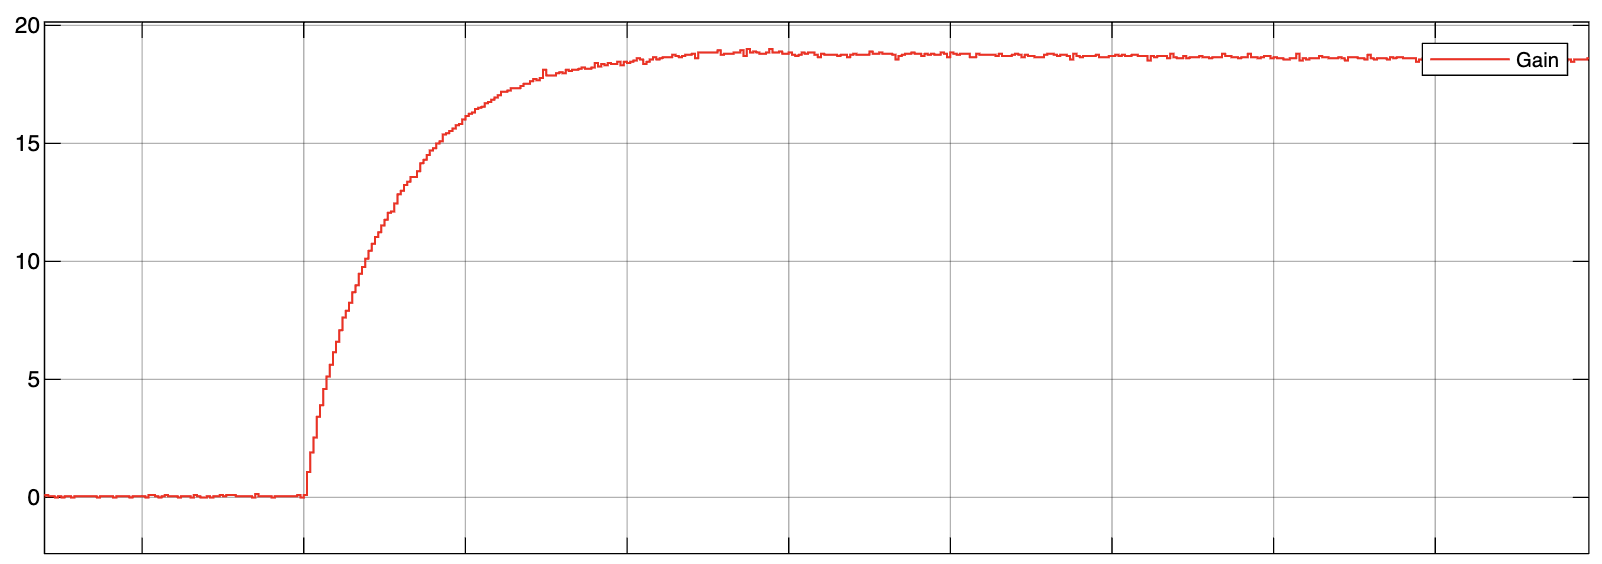
\includegraphics[width=0.7\textwidth]{figures/graph_i_time.png}
\caption{Current response $I(t)$ to step voltage input, showing the transient behavior and steady-state value.}
\label{fig:i_time}
\end{figure}

Thus, from the steady-state and transient measurements, the armature resistance and inductance of the DC machine were found to be:

\[
R = 0.3504~\Omega, \qquad L = 0.00876~\mathrm{H}.
\]

These values will be used in subsequent stages for the modeling and control design of the electrical drive system.

\subsection{Voltage Constant and Torque Constant: $K_e = K_c$}

In steady state, the armature voltage satisfies
\[
U_m = E + R\,I = K_e\,\Omega + R\,I,
\]
so the (back–EMF) voltage constant $K_e$ (equal to the torque constant $K_c$ in SI units) can be obtained directly from averaged steady-state measurements as
\[
K_e \;=\; \frac{\overline{U}_m - R\,\overline{I}}{\overline{\Omega}} \qquad (\text{with } \overline{\Omega}\text{ in rad/s}).
\]


\paragraph{}
With the rotor turning (stator energized), we applied a constant control $u_c$ at the converter input and increased it in steps $u_c=0,2,3,4~\mathrm{V}$, waiting for steady state each time. At steady state we recorded:
(i) the average armature voltage $U_m$ (voltmeter),
(ii) the current sensor output $V_I$ (converted to $I$ via $I=V_I/K_{\mathrm{cap}I}$ with $K_{\mathrm{cap}I}=0.1~\mathrm{V/A}$),
and (iii) the rotational speed in rpm (converted to $\Omega$ via $\Omega= \text{rpm}\cdot 2\pi/60$).

\paragraph{}
\begin{table}[H]
\centering
\caption{Steady-state measurements and converted quantities.}
\label{tab:Ke_data}
\begin{tabular}{lccccc}
\toprule
$u_c$ (V) & $V_I$ (V) & rpm & $\Omega$ (rad/s) & $I=V_I/0.1$ (A) & $U_m$ (V)\\
\midrule
0 & 0.0374 & 3.0184  & 0.316086 & 0.374  & 0 \\
2 & 0.9976 & 57.1736 & 5.987205 & 9.976  & 5 \\
3 & 1.1536 & 184.3761& 19.307820& 11.536 & 16 \\
4 & 1.2517 & 317.6292& 33.262052& 12.517 & 27 \\
\bottomrule
\end{tabular}
\end{table}

Using the previously identified armature resistance
\[
R = 0.350404313~\Omega,
\]
and the averaged values from our measurements (already converted to SI units):
\[
\overline{U}_m = 12~\text{V},\quad
\overline{I} = 0.860075~\text{A},\quad
\overline{\Omega} = 14.7182909~\text{rad/s} \;\;(\text{from } 140.549325~\text{rpm}),
\]
we obtain
\[
K_e \;=\; \frac{12 - 0.350404313 \times 0.860075}{14.7182909}
\;=\; 0.794835901~\text{V}\cdot\text{s/rad}.
\]

Hence, in SI units,
\[
\boxed{\,K_e = K_c \approx 0.794835901~\text{V}\cdot\text{s/rad}\,}.
\]

\subsection{Coulomb Friction Torque and Viscous Friction Coefficient: $C_s$ and $f$}

In steady state (constant speed, $\dot{\Omega}=0$) and with zero external load torque ($C_r=0$), the DC motor torque balance reduces to
\[
K_c\,I \;=\; f\,\Omega \;+\; C_s ,
\]
where $K_c$ is the torque constant (equal to the back–EMF constant in SI), $f$ is the viscous friction coefficient, and $C_s$ is the Coulomb (dry) friction torque.

Hence, plotting the measured current $I$ versus angular speed $\Omega$ and fitting the affine model
\[
I \;=\; a\,\Omega \;+\; b
\]
yields $f = K_c\,a$ and $C_s = K_c\,b$.

\paragraph{}
\begin{table}[H]
\centering
\caption{Steady-state points used for $I$–$\Omega$ identification.}
\label{tab:friction_data}
\begin{tabular}{lcccc}
\toprule
$u_c$ (V) & $U_m$ (V) & rpm & $\Omega$ (rad/s) & $I$ (A)\\
\midrule
2 & 5  & 57.1736  & 5.987205 & 0.9976 \\
3 & 16 & 184.3761 & 19.307820 & 1.1536 \\
4 & 27 & 317.6292 & 33.262052 & 1.2517 \\
6 & 49 & 593.3711 & 62.137676 & 1.6074 \\
\bottomrule
\end{tabular}
\end{table}

A linear regression of $I$ vs.\ $\Omega$ gives (see plotted trendline):
\[
I \;=\; \underbrace{0.0107}_{a}\,\Omega \;+\; \underbrace{0.9293}_{b}\quad [\mathrm{A}],
\]
with $\Omega$ in rad/s.

\begin{figure}[H]
\centering
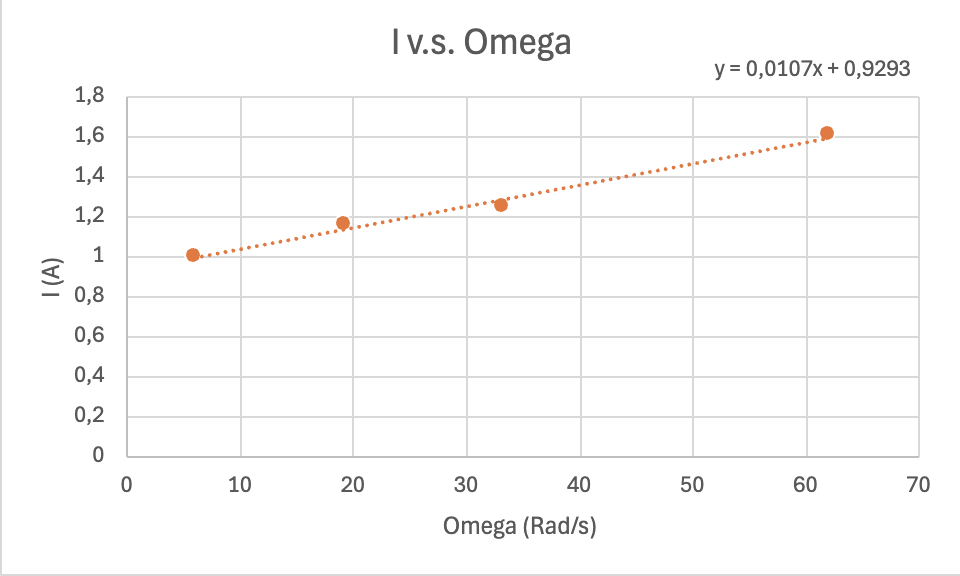
\includegraphics[width=0.7\textwidth]{figures/graph_i_omega.png}
\caption{Linear regression of steady-state current $I$ versus angular speed $\Omega$.}
\label{fig:i_omega}
\end{figure}

Using the previously identified $K_c = K_e = 0.794835901~\mathrm{V\,s/rad} = \mathrm{N\,m/A}$, we obtain
\[
f \;=\; K_c\,a \;=\; 0.794835901 \times 0.0107 \;=\; \mathbf{0.008504744}~\mathrm{N\,m\,s},
\]
\[
C_s \;=\; K_c\,b \;=\; 0.794835901 \times 0.9293 \;=\; \mathbf{0.738641003}~\mathrm{N\,m}.
\]

These friction parameters will be used in the motor model and subsequent controller design/validation.

\subsection{Moment of Inertia of the System: $J$}

When the control signal is removed, the motor supply is cut and the rotor slows down under the effect of friction only. The dynamic equation governing the deceleration is:
\[
J\,\dot{\Omega} + f\,\Omega + C_s = 0,
\]
which can be written as:
\[
\dot{\Omega} + \frac{1}{\tau}\,\Omega = -\frac{C_s}{J}, \qquad \text{with } \tau = \frac{J}{f}.
\]
The solution of this first-order differential equation is:
\[
\Omega(t) = \left(\Omega_0 + \frac{C_s}{f}\right)e^{-t/\tau} - \frac{C_s}{f},
\]
where $\Omega_0$ is the speed at the moment the supply is interrupted.

\begin{figure}[H]
\centering
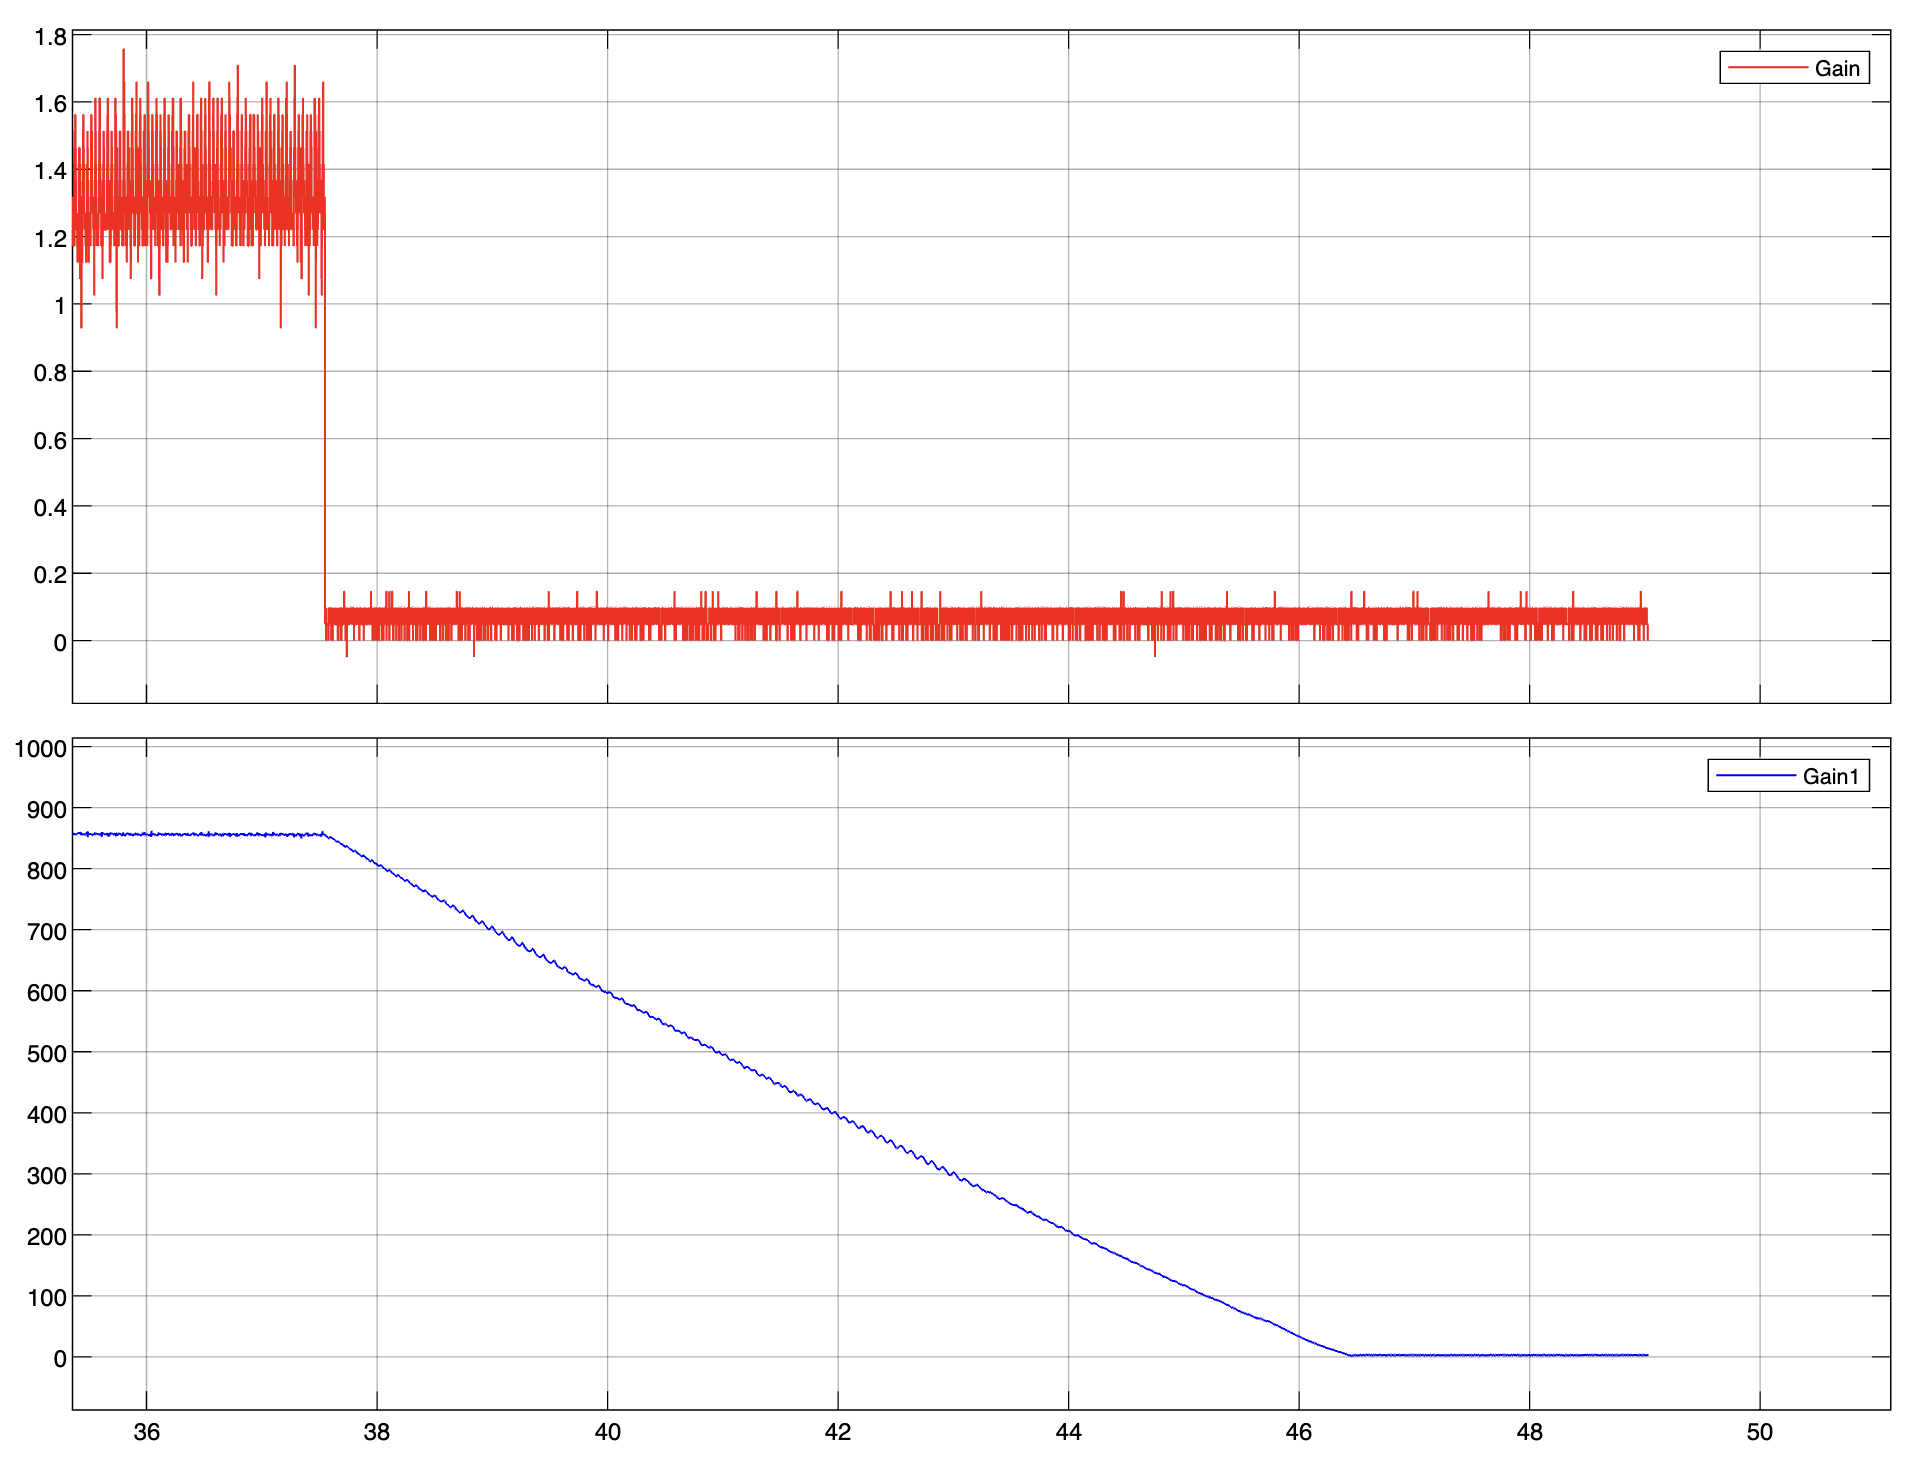
\includegraphics[width=0.7\textwidth]{figures/signal_removed.png}
\caption{Angular velocity $\Omega(t)$ decay (blue curve) when the control signal is removed, showing exponential deceleration due to friction.}
\label{fig:J_measurement}
\end{figure}

From the experimental speed curve (see Figure~\ref{fig:J_measurement}), the motor exhibits an exponential decay in velocity until it comes to rest. By determining the time constant $\tau$ from the slope of this decay, the moment of inertia is obtained as:
\[
J = \tau\,f.
\]
Using the identified viscous friction coefficient and the time constant estimated from the measured response, we find:
\[
\boxed{J = 0.1213266~\mathrm{kg\cdot m^2}}.
\]

This value will be used in the subsequent modeling and simulation stages to complete the characterization of the DC motor’s mechanical dynamics.



\newpage
%------------ Section 2 ----------------

\section{Controller Design and Validation by Simulations}
\lipsum[4-6]





\newpage
%------------ Section 3 ----------------

\section{Experimental Validation of the Controllers}

\label{sec:exp}

This section reports the laboratory validation of the controllers designed in Part~2. 
Several Simulink configurations were used successively (current loop, speed loop, and finally the observer). 
Due to limited laboratory time, \textbf{only the final implementation corresponding to the observer (Part~3.3) was saved as a representative Simulink diagram}. 
However, \textbf{all measurement results} obtained at each step were recorded and are presented below to assess the performance of every loop. 
Earlier configurations for the current and speed control followed the same structure as the final one (inner current loop, outer speed loop, voltage saturation, and acquisition blocks).

\vspace{4pt}
\noindent\textit{Practical constraints.} For hardware safety, the armature current was limited to 20~A, voltage commands were saturated at $\pm9$~V, and step amplitudes were increased gradually to avoid excessive mechanical stress and large current transients.

%-------------------- 3.1 --------------------
\subsection{Current Regulation Experiment}

The experimental results of the current control loop are shown in Figure~\ref{fig:exp_I_20A}. 
The upper plot displays the armature current (\textit{courant}) and the lower plot shows the corresponding motor speed (\textit{vitesse}). 
Several step changes were applied to the current reference, increasing successively from approximately 1~A to 2~A, 3~A and finally 10~A. 
The current follows the reference with a fast transient and negligible overshoot, demonstrating a well-tuned inner current loop. 
Small fluctuations in the measured signal are mainly due to sensor noise. 
The motor speed evolves consistently with the current variations, rising up to about 1000~rpm and then decreasing when the current is reduced or reversed. 
This confirms the expected electromechanical coupling between torque and speed. 
At the end of the experiment, both current and speed return smoothly to zero when the converter command is disabled.

\begin{figure}[H]
    \centering
    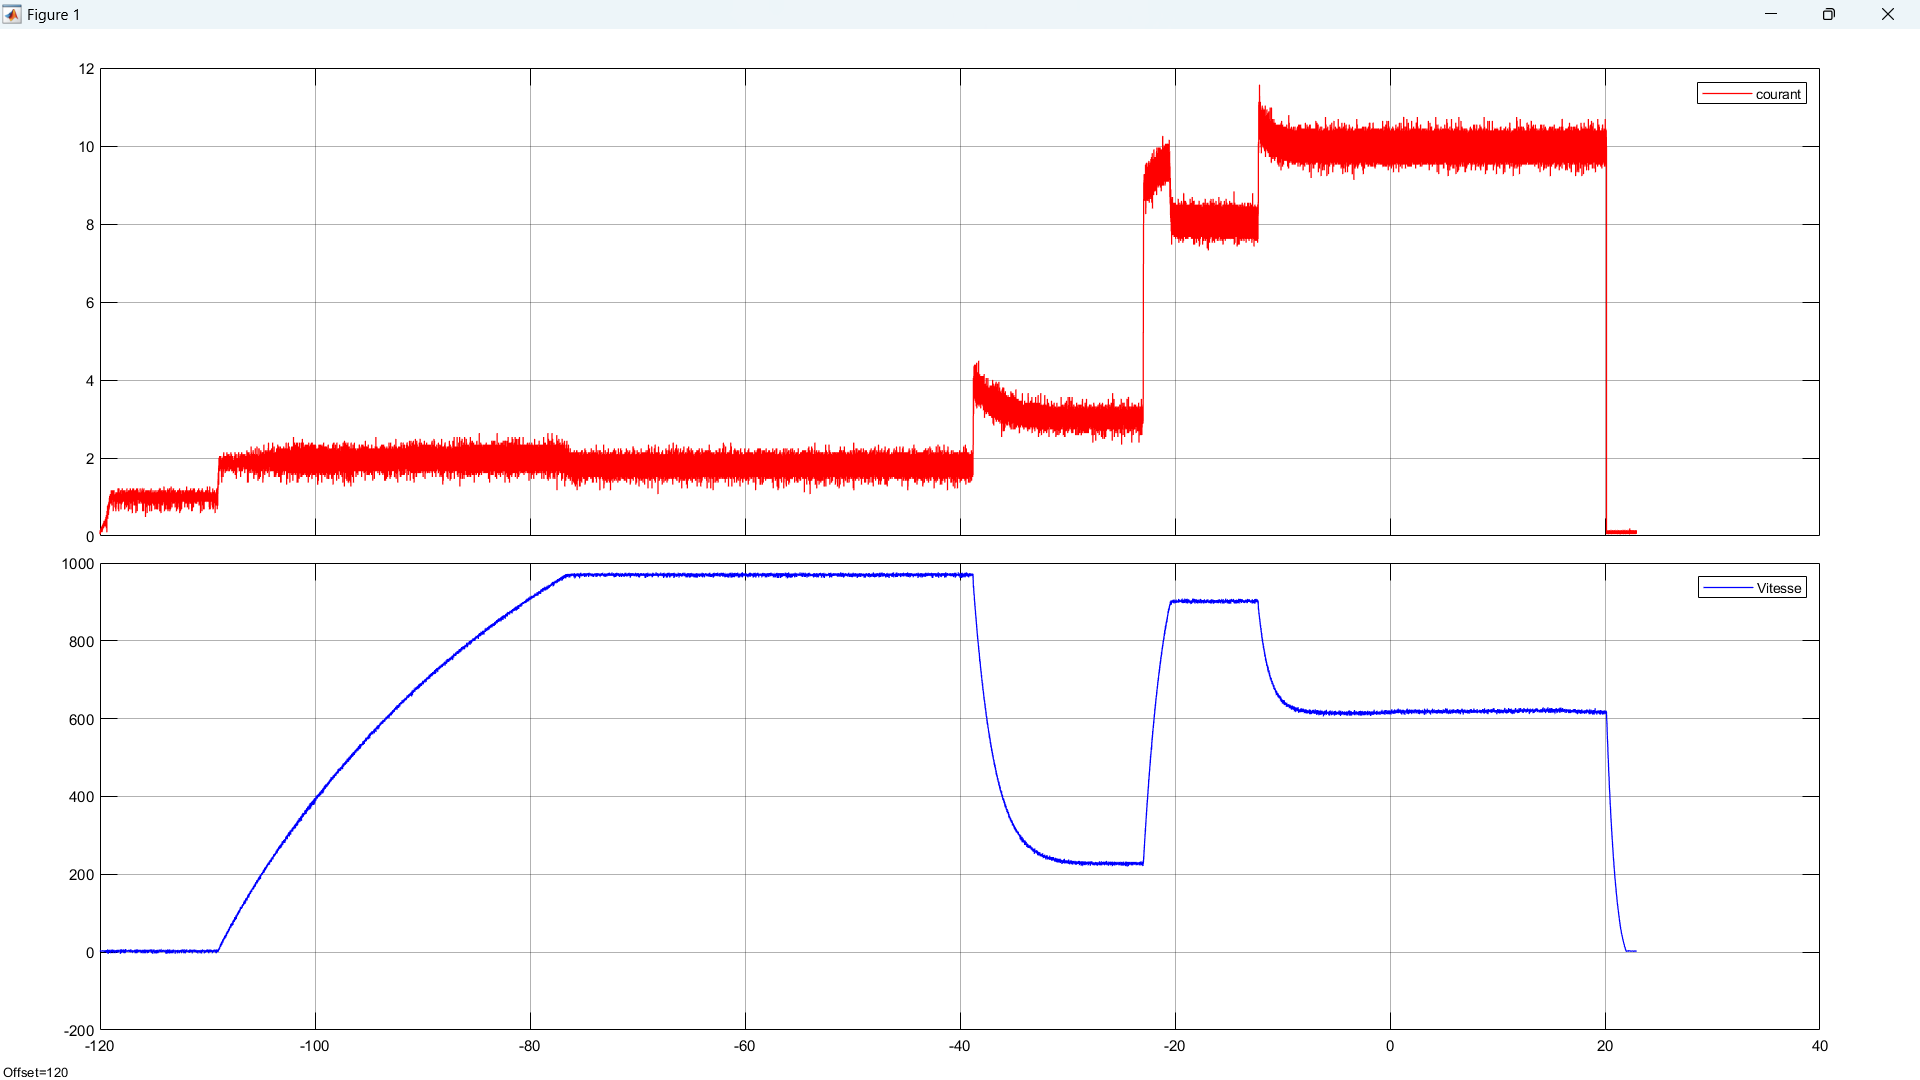
\includegraphics[width=\linewidth, keepaspectratio]{figures/PP1.png}
    \caption{Measured current (top, in~A) and speed (bottom, in~rpm) during the current regulation test. 
    The current loop shows fast and stable response with negligible overshoot.}
    \label{fig:exp_I_20A}
\end{figure}


%-------------------- 3.2 --------------------
\subsection{Speed Regulation Experiment}

The experimental validation of the speed controller was performed following the four test scenarios defined in Question~2.2.c. 
For each case, the converter operated in ``Automatic'' mode, and the speed reference $\Omega^*(t)$ was imposed through the control panel. 
The measured motor speed (\textit{vitesse}) and armature current (\textit{courant}) were recorded simultaneously.

\begin{itemize}
    \item $\mathbf{Case~1:}$ $C_r(t)=0$, $\Omega^*(t)$ changes from $0$ to $300~\text{rpm}$ at $t=1~\text{s}$.
    \item $\mathbf{Case~2:}$ $C_r(t)=0$, $\Omega^*(t)$ changes from $0$ to $500~\text{rpm}$ at $t=1~\text{s}$.
    \item $\mathbf{Case~3:}$ $C_r(t)=0$, $\Omega^*(t)$ changes from $0$ to $1200~\text{rpm}$ at $t=1~\text{s}$.
    \item $\mathbf{Case~4:}$ $\Omega^*(t)$ changes from $0$ to $300~\text{rpm}$ at $t=1~\text{s}$, while the resistant torque $C_r(t)$ increases from $0$ to $5~\text{Nm}$ at $t=10~\text{s}$.
\end{itemize}

The measured responses are summarized in Figures~\ref{fig:exp_W_300}--\ref{fig:exp_W_disturbance}. 
In all cases, the speed regulation shows a well-damped transient with limited overshoot and negligible steady-state error. 
For moderate speed commands (300~rpm and 500~rpm), the current peaks remain within the admissible range (below 20~A), confirming that the current limiter effectively constrains the torque demand. 
When the reference is increased to 1200~rpm, the system still converges but the transient becomes slower, illustrating the saturation effect of the voltage converter.

When a disturbance torque of 5~Nm is applied at $t=10~\text{s}$, a brief speed drop is observed, immediately compensated by the integral action of the speed controller. 
The steady-state speed returns to its nominal value within less than one second, demonstrating the robustness of the closed-loop regulation against load disturbances.

\begin{figure}[H]
    \centering
    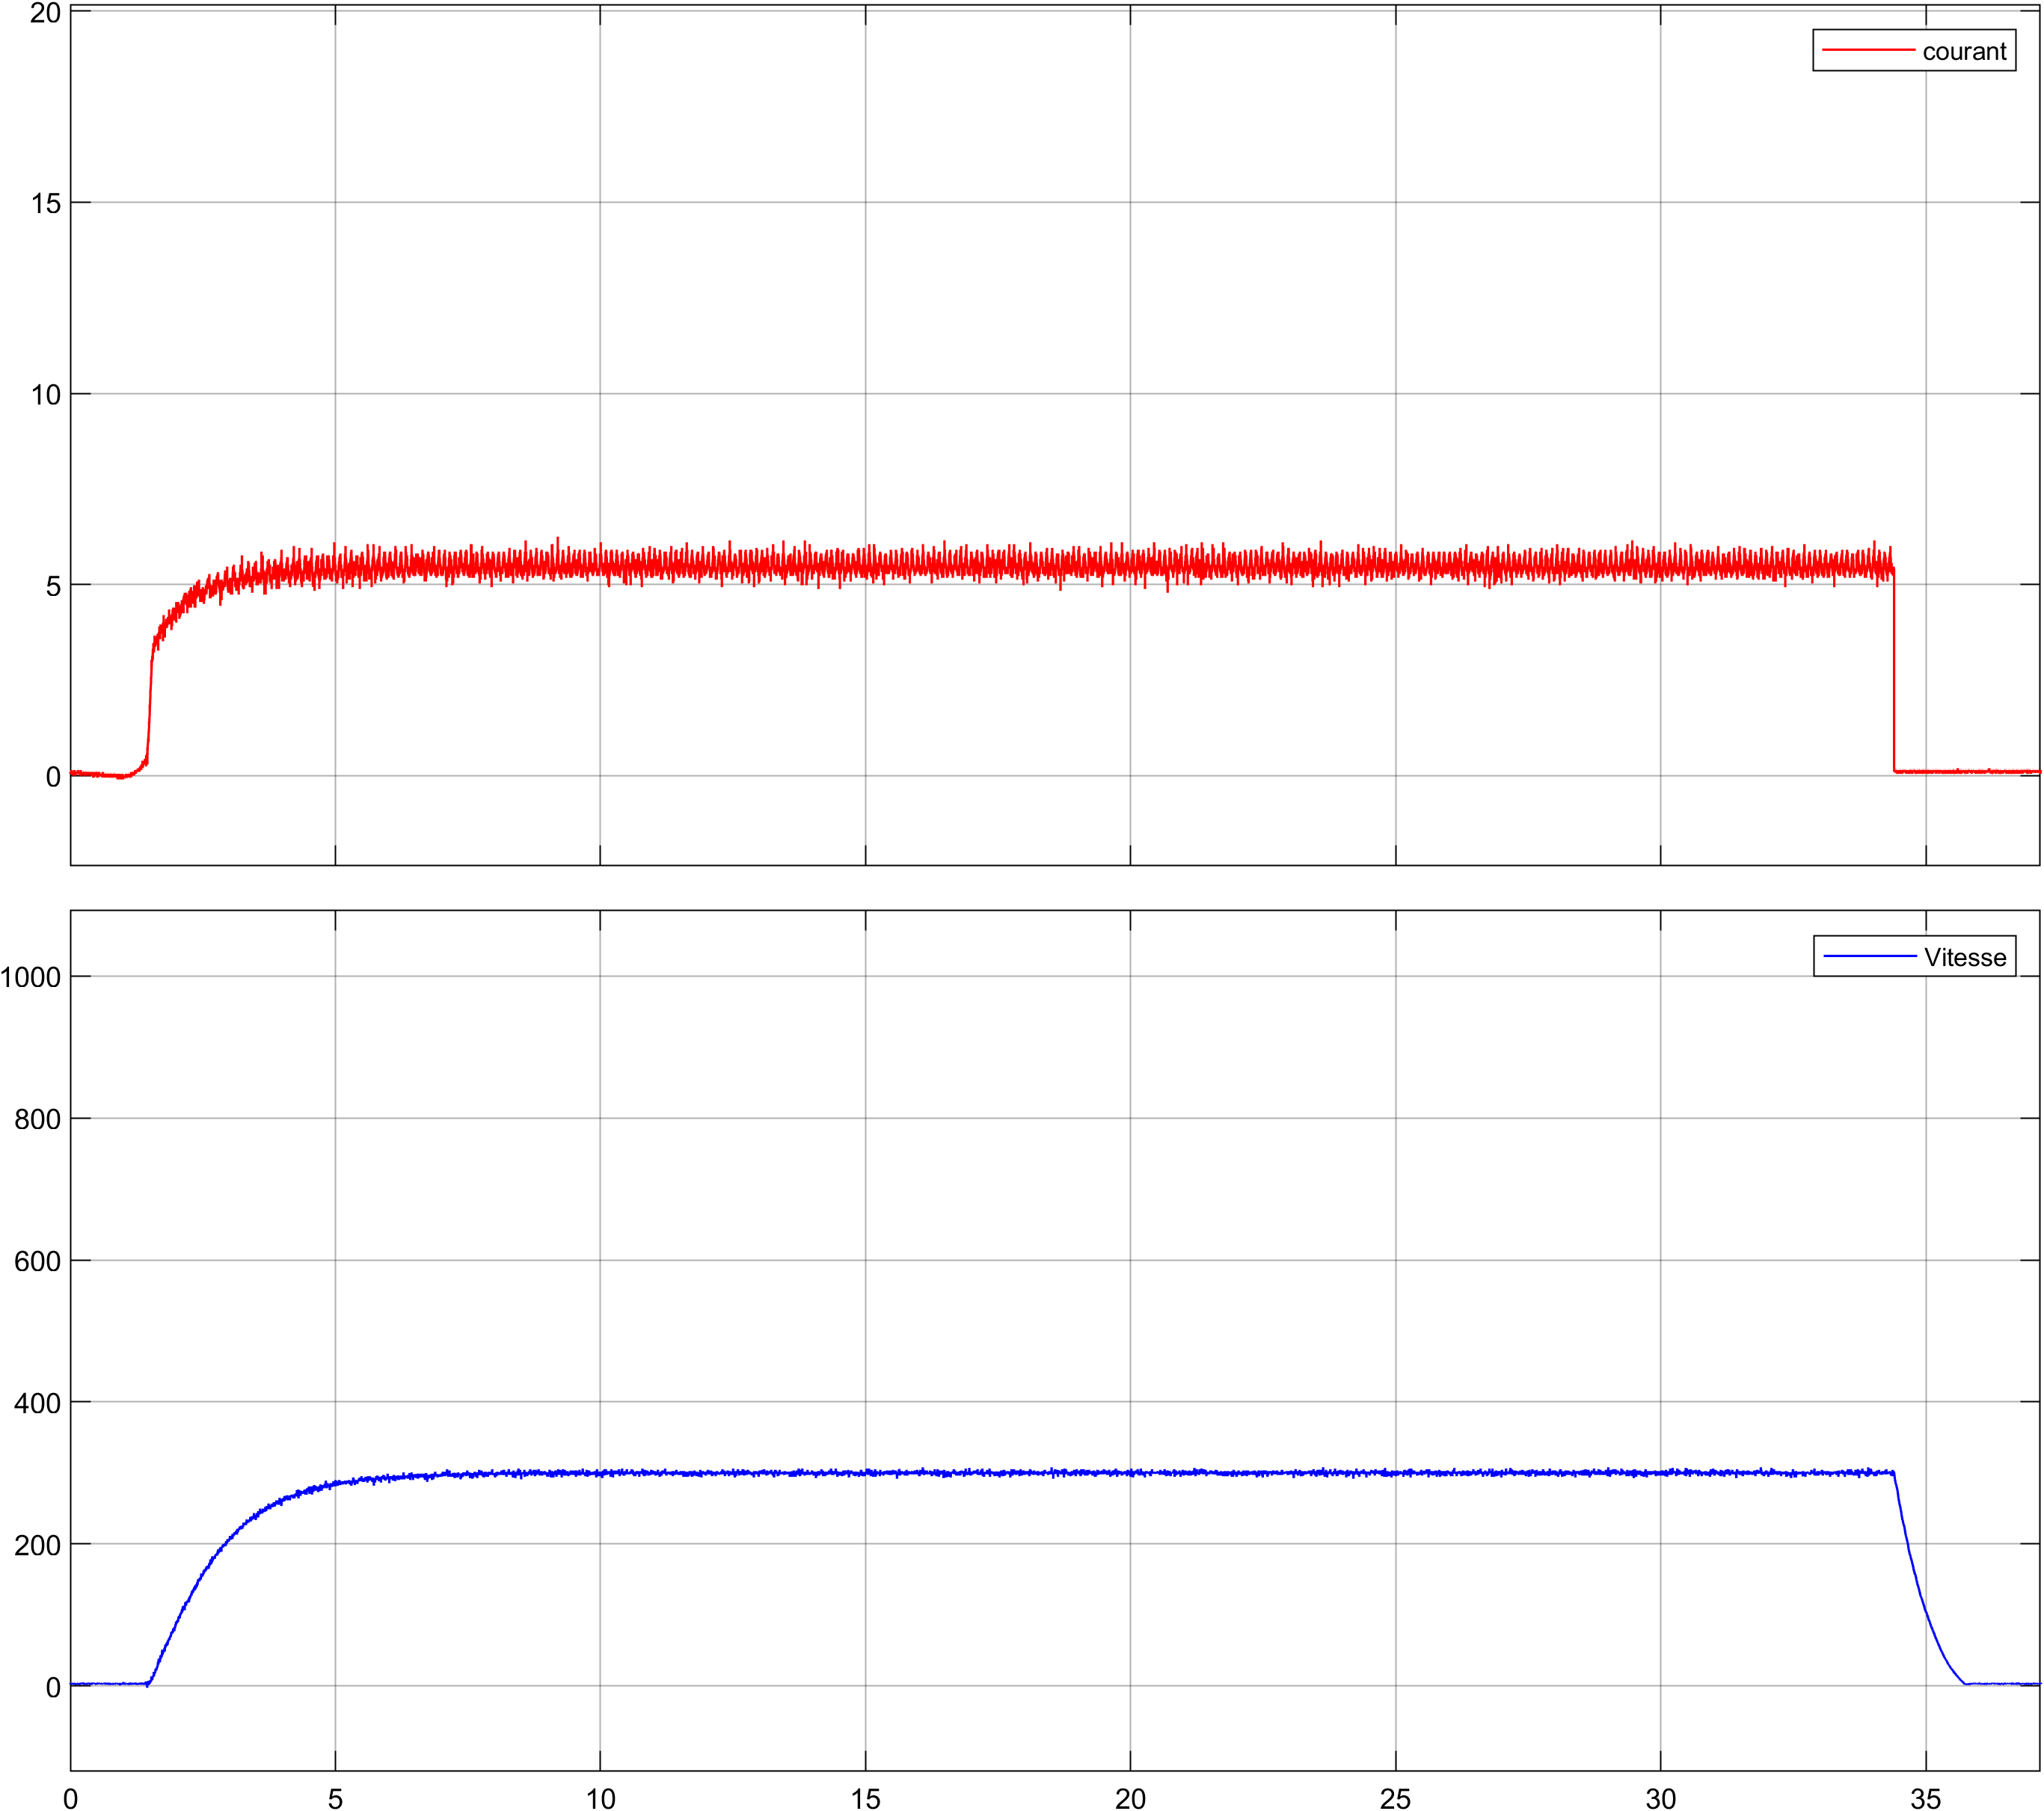
\includegraphics[width=\linewidth, keepaspectratio]{figures/p300.png}
    \caption{Speed loop --- measured response for a $0 \rightarrow 300~\text{rpm}$ reference step.}
    \label{fig:exp_W_300}
\end{figure}

\begin{figure}[H]
    \centering
    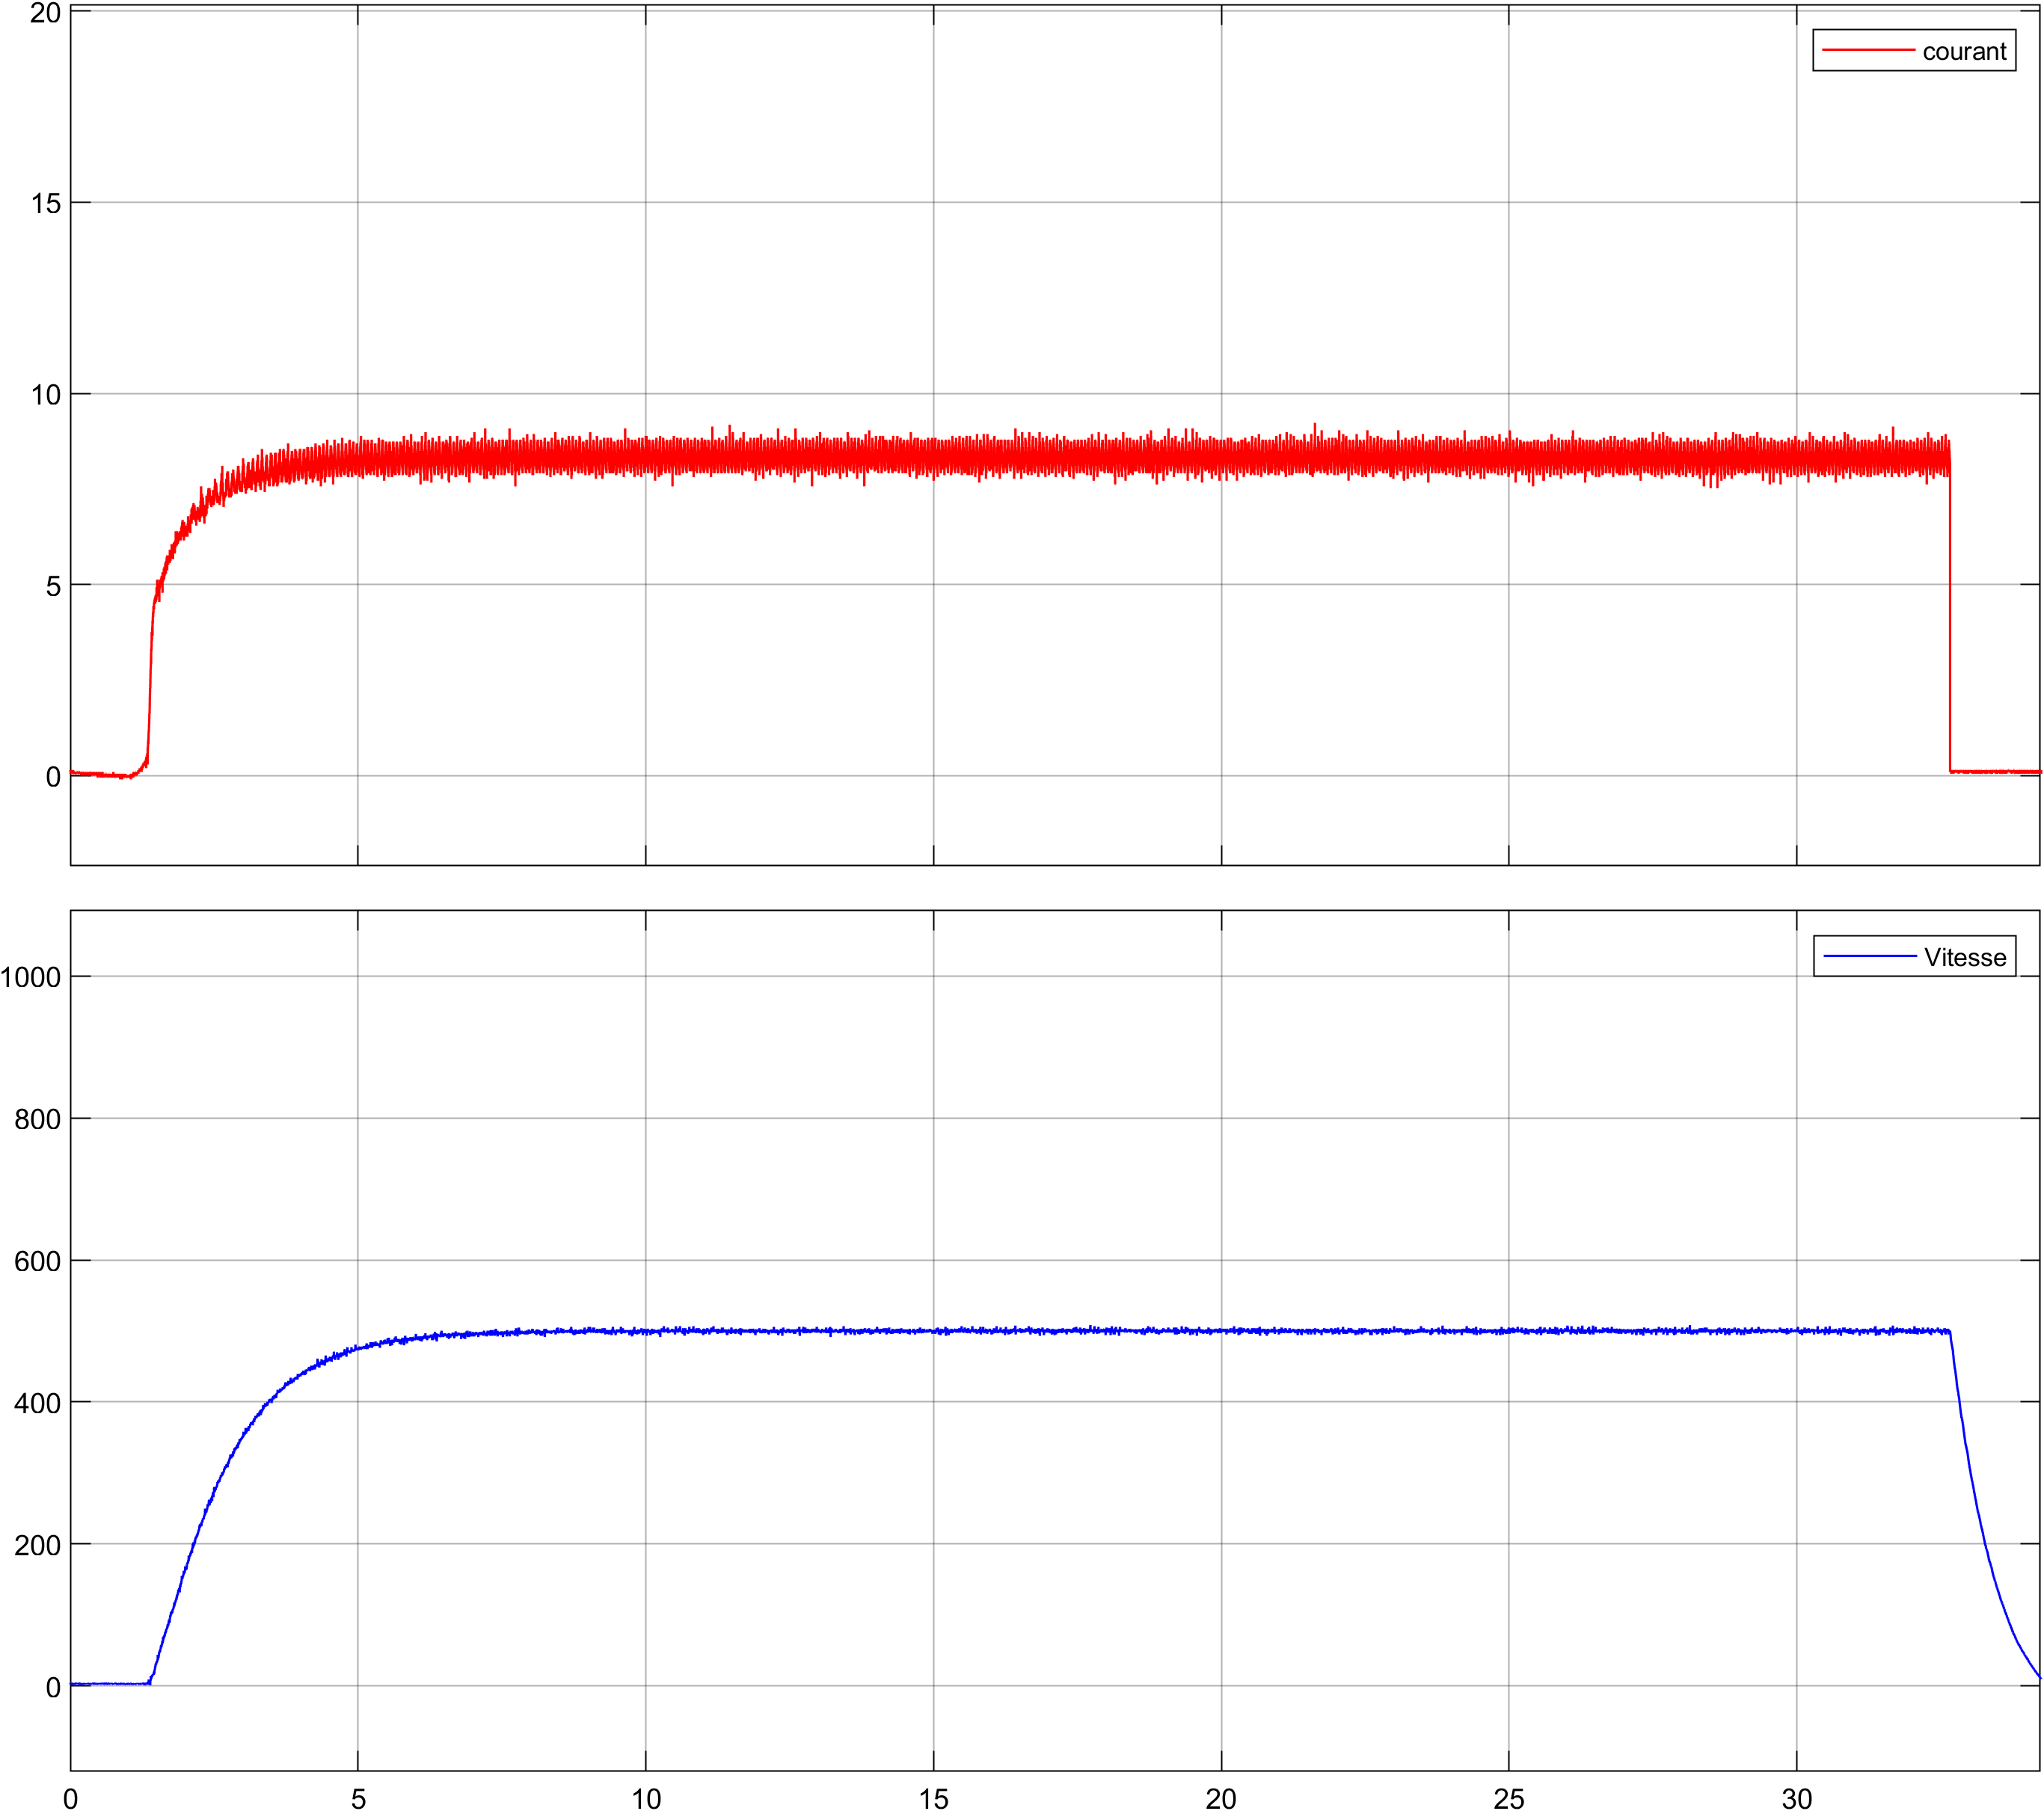
\includegraphics[width=\linewidth, keepaspectratio]{figures/p500.png}
    \caption{Speed loop --- measured response for a $0 \rightarrow 500~\text{rpm}$ reference step.}
    \label{fig:exp_W_500}
\end{figure}

\begin{figure}[H]
    \centering
    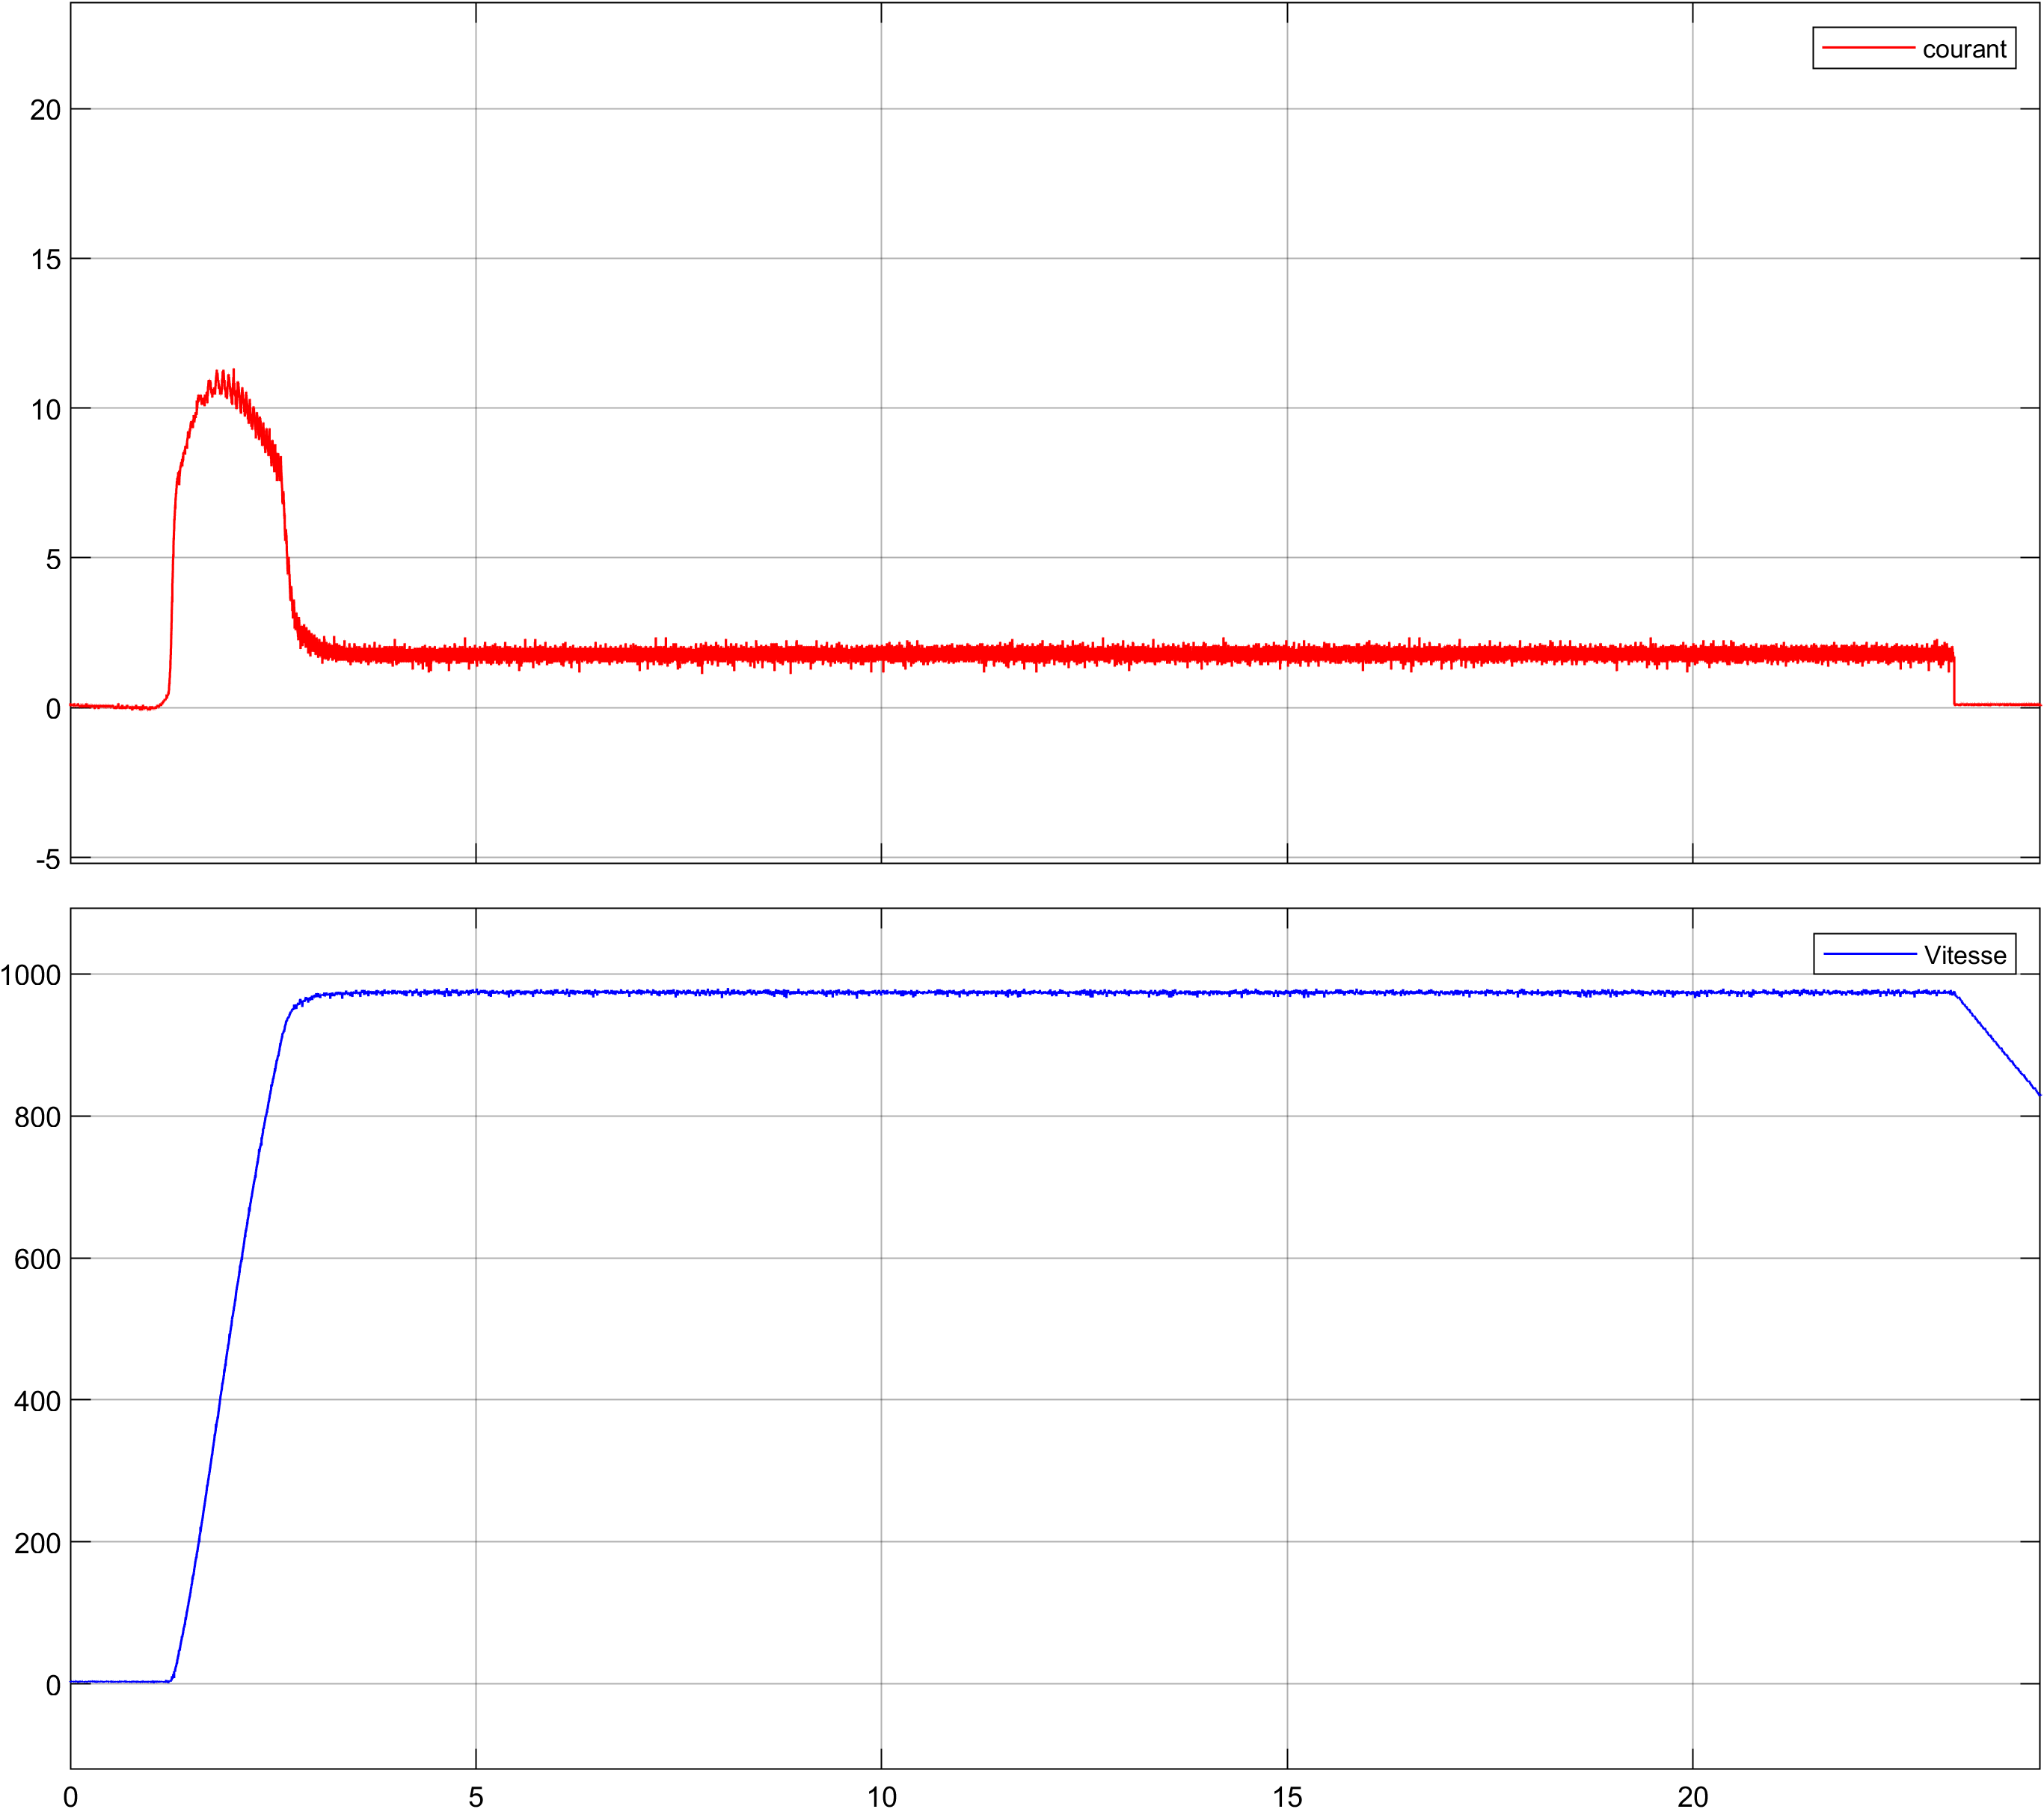
\includegraphics[width=\linewidth, keepaspectratio]{figures/p1200.png}
    \caption{Speed loop --- measured response for a $0 \rightarrow 1200~\text{rpm}$ reference step, showing converter saturation effects.}
    \label{fig:exp_W_1200}
\end{figure}

\begin{figure}[H]
    \centering
    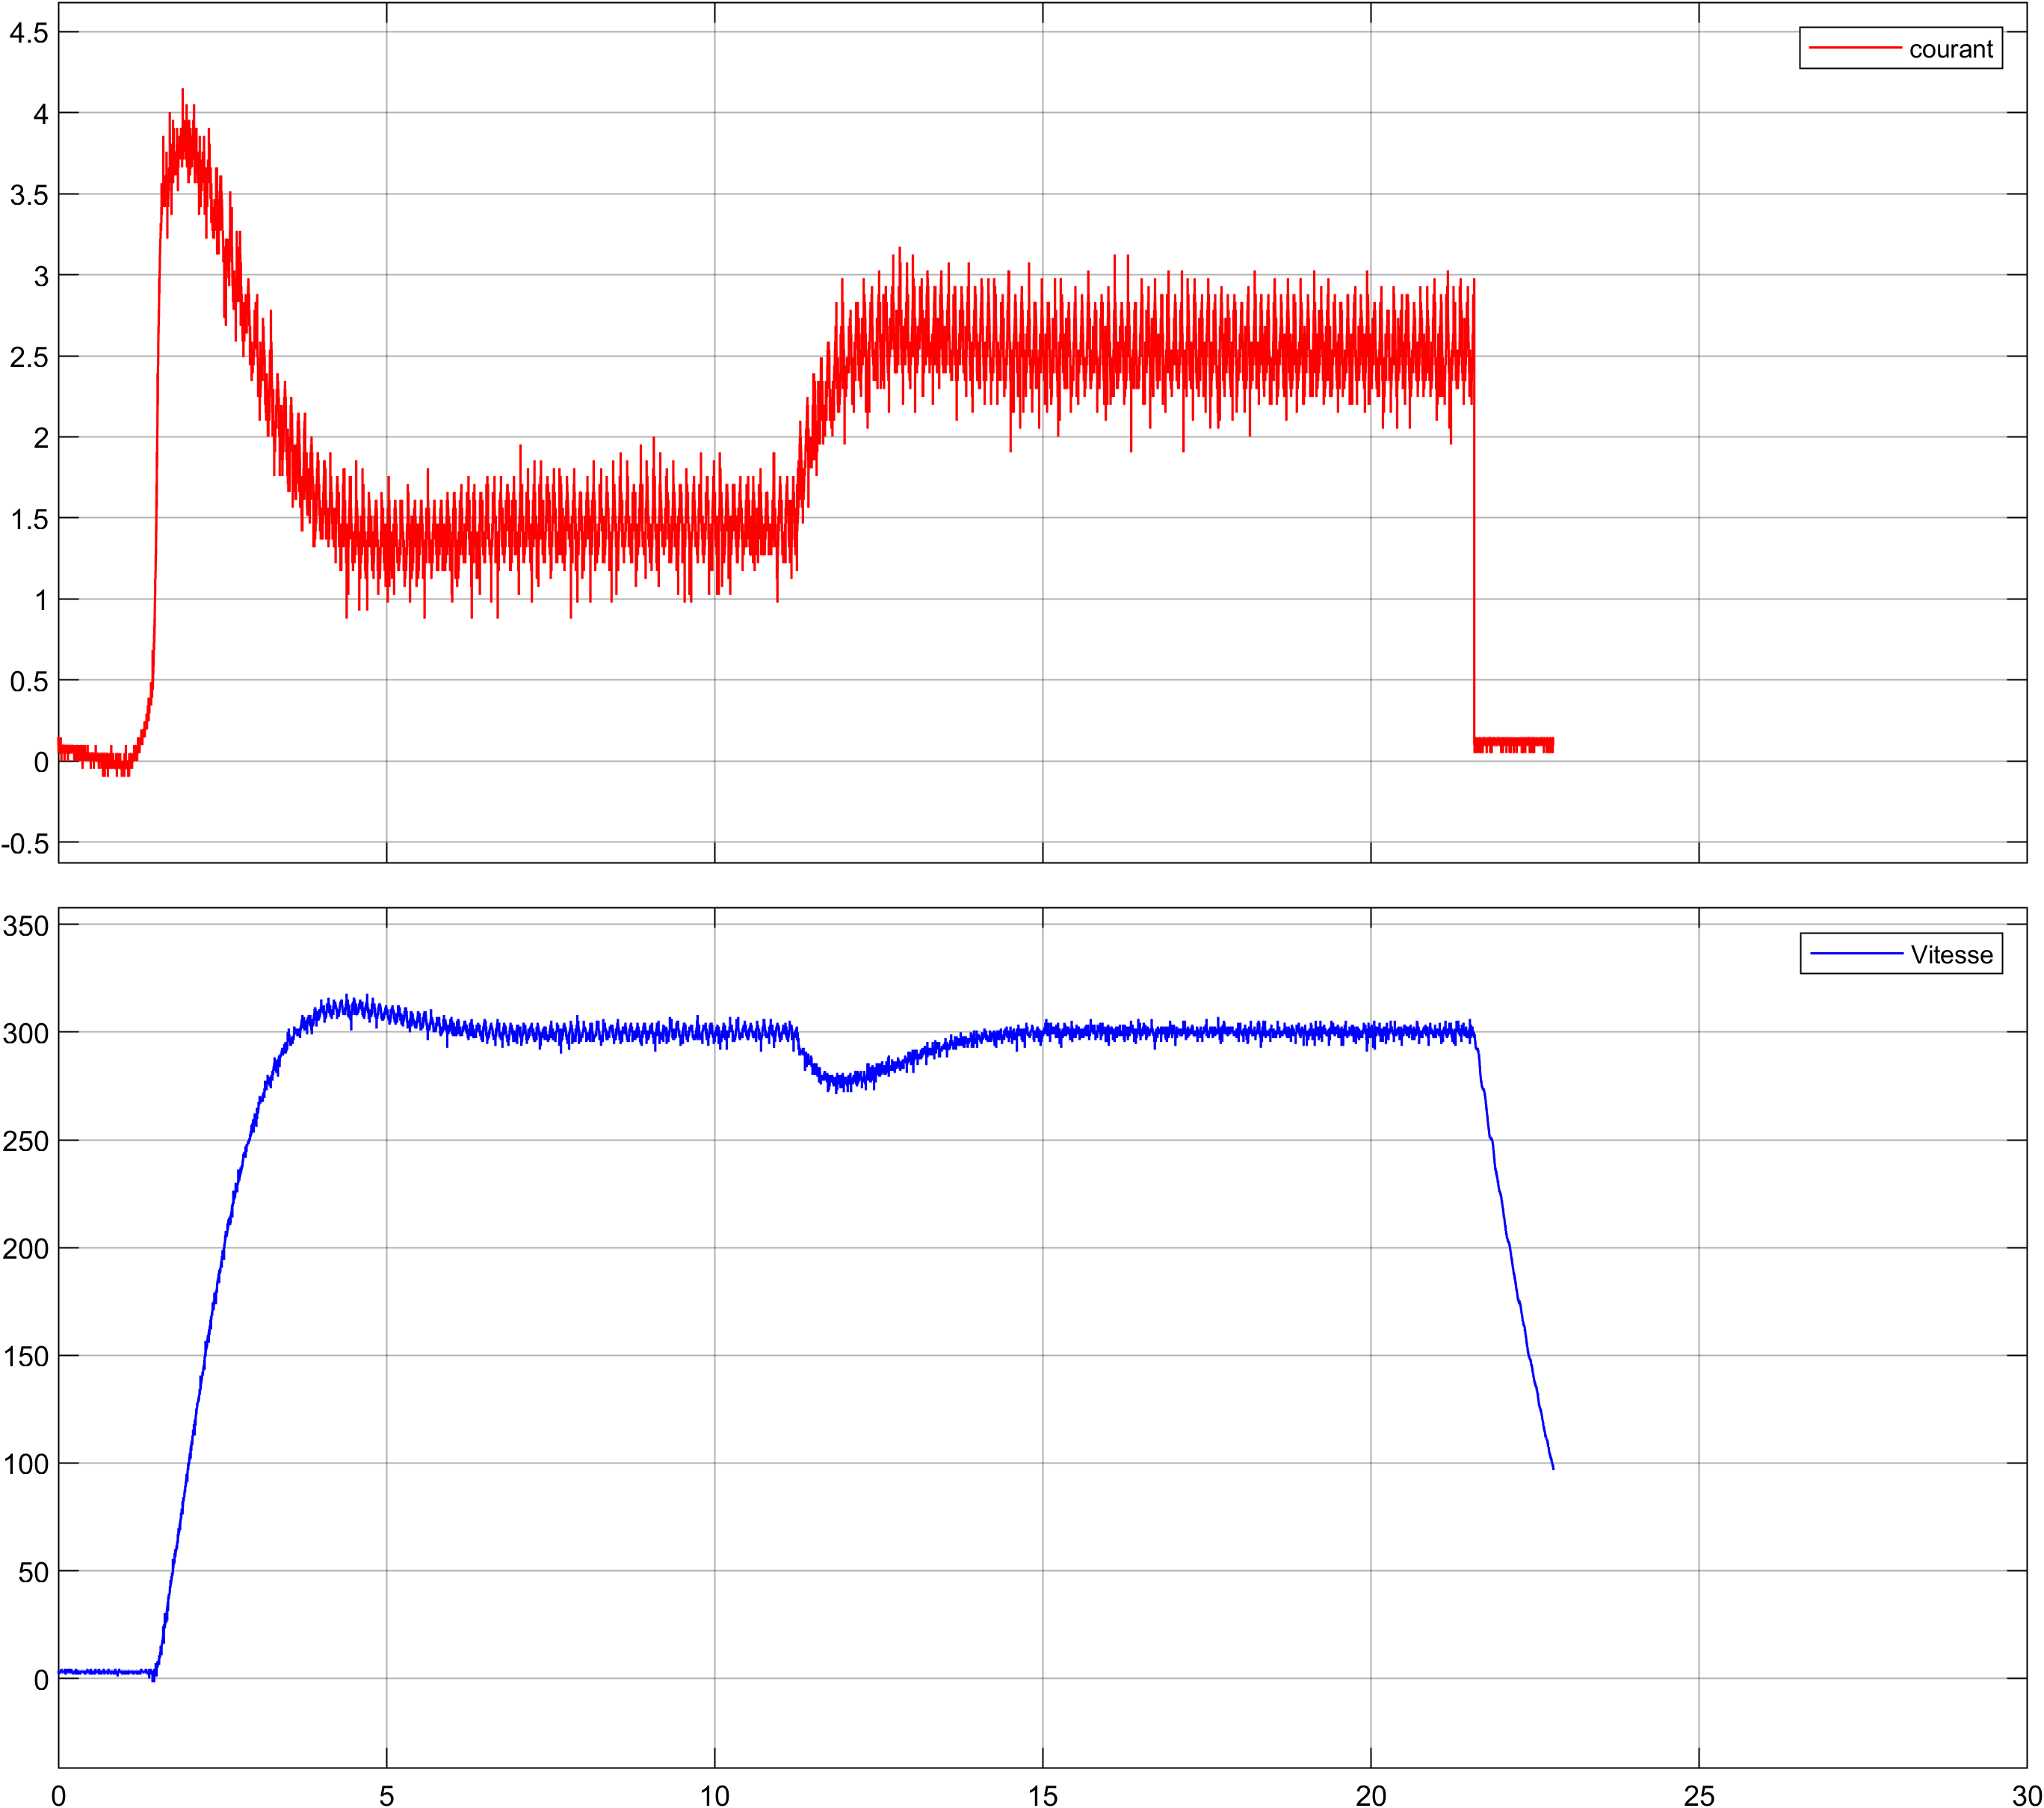
\includegraphics[width=\linewidth, keepaspectratio]{figures/p300cr5.png}
    \caption{Speed loop --- disturbance rejection test: a $5~\text{Nm}$ torque is applied at $t=10~\text{s}$. 
    The controller compensates the perturbation and restores the nominal speed.}
    \label{fig:exp_W_disturbance}
\end{figure}

%-------------------- 3.3 --------------------
\subsection{Observer Implementation and Validation}
\label{subsec:exp_obs}

Finally, the observer developed in Section~2.3 was implemented to estimate the states $[\hat I,\ \hat\Omega,\ \hat C_r]$. 
The \textbf{final Simulink configuration} used for all experiments is shown in Figure~\ref{fig:exp_obs_model}; it summarizes the complete control architecture (inner current loop, outer speed loop, observer, saturation, and I/O blocks).

\begin{figure}[H]
    \centering
    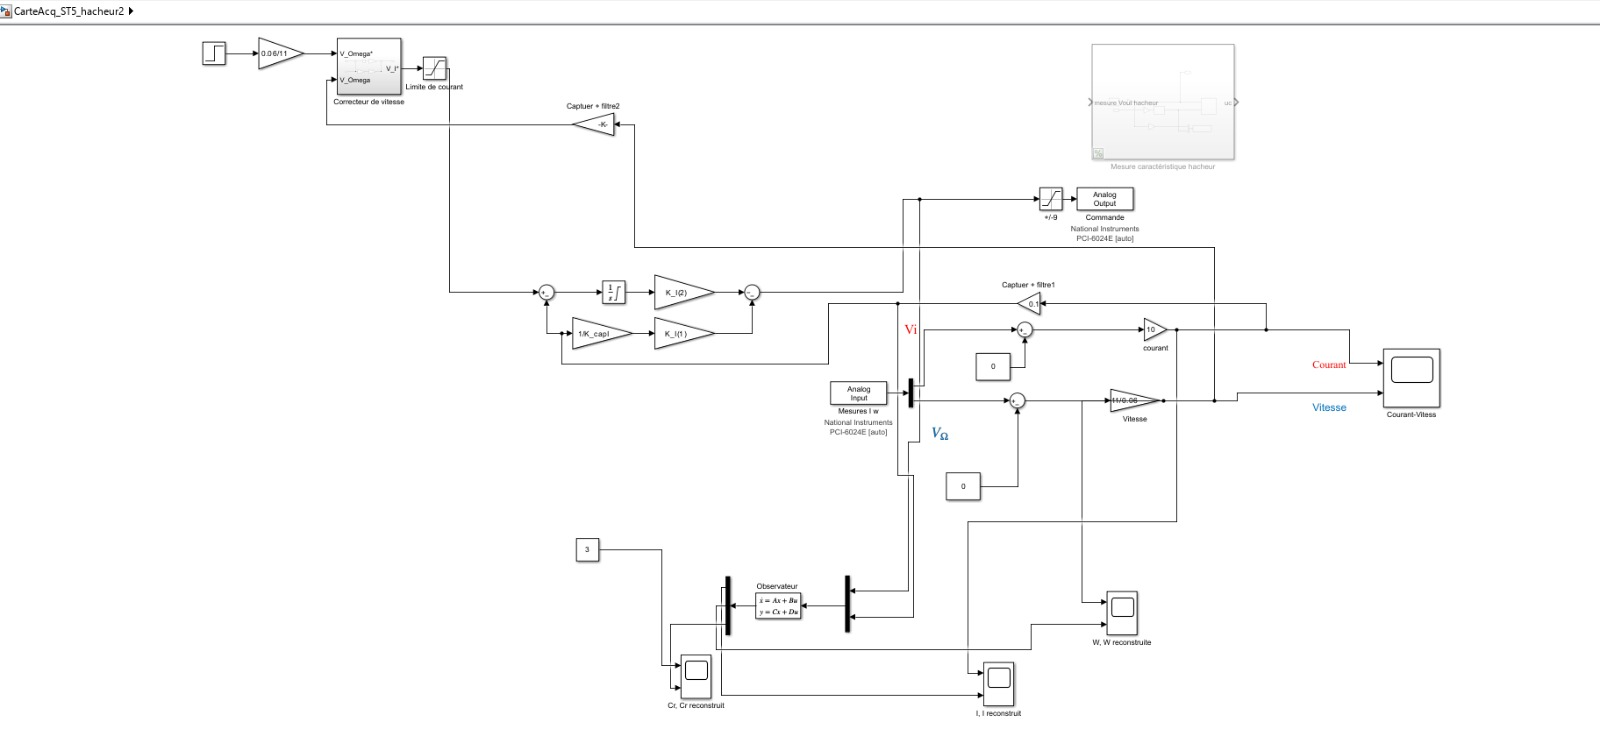
\includegraphics[width=\linewidth, keepaspectratio]{figures/simulink.png}
    \caption{Final Simulink implementation used on the bench (saved during Part~3.3). 
    Earlier configurations for the current and speed loops followed the same structure.}
    \label{fig:exp_obs_model}
\end{figure}

The current estimate converged rapidly and accurately. 
The speed estimate showed small mismatches and high-frequency noise, mainly due to sensor noise and converter nonlinearities. 
When using $\hat C_r$ for proportional disturbance compensation, the closed loop became sensitive to this noise and could lose stability. 
Therefore, compensation based on $\hat C_r$ was not retained on the bench without additional filtering or gain scheduling. 
Figure~\ref{fig:exp_obs_results} illustrates the convergence of the estimated variables towards their measured counterparts.

\begin{figure}[H]
    \centering
    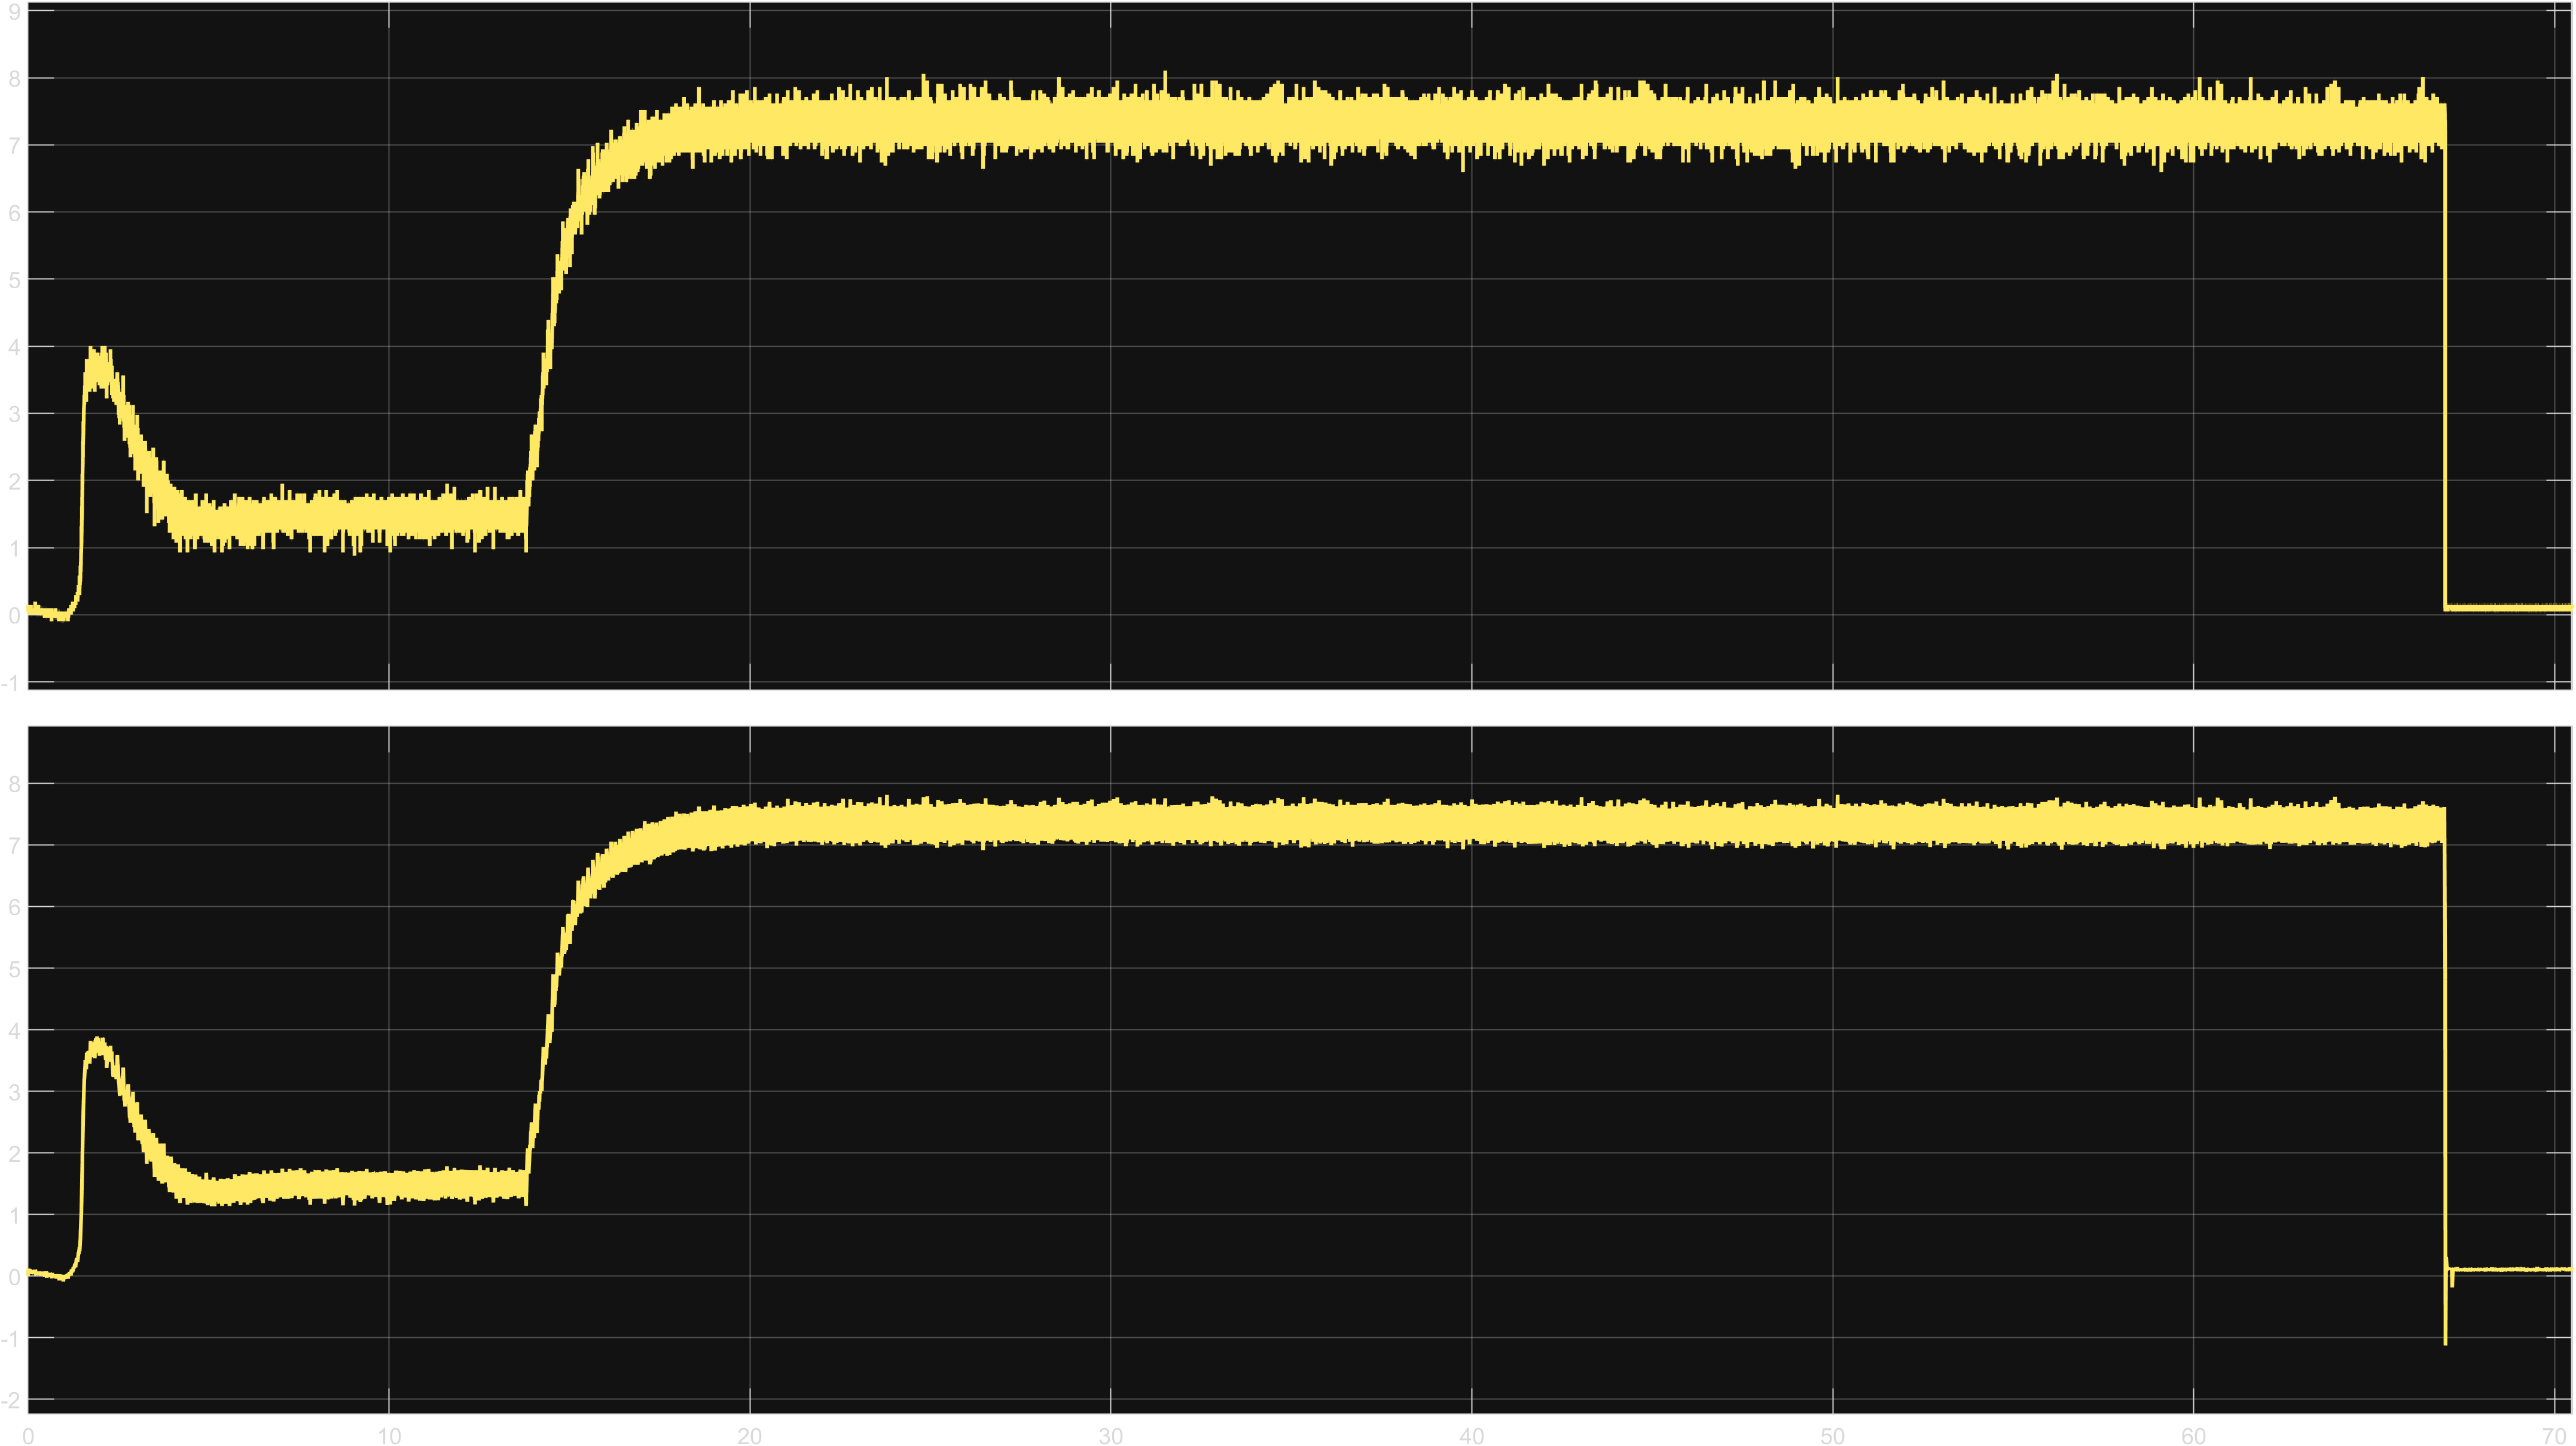
\includegraphics[width=\linewidth, keepaspectratio]{figures/p3i.png}
    \vspace{0.5em}
    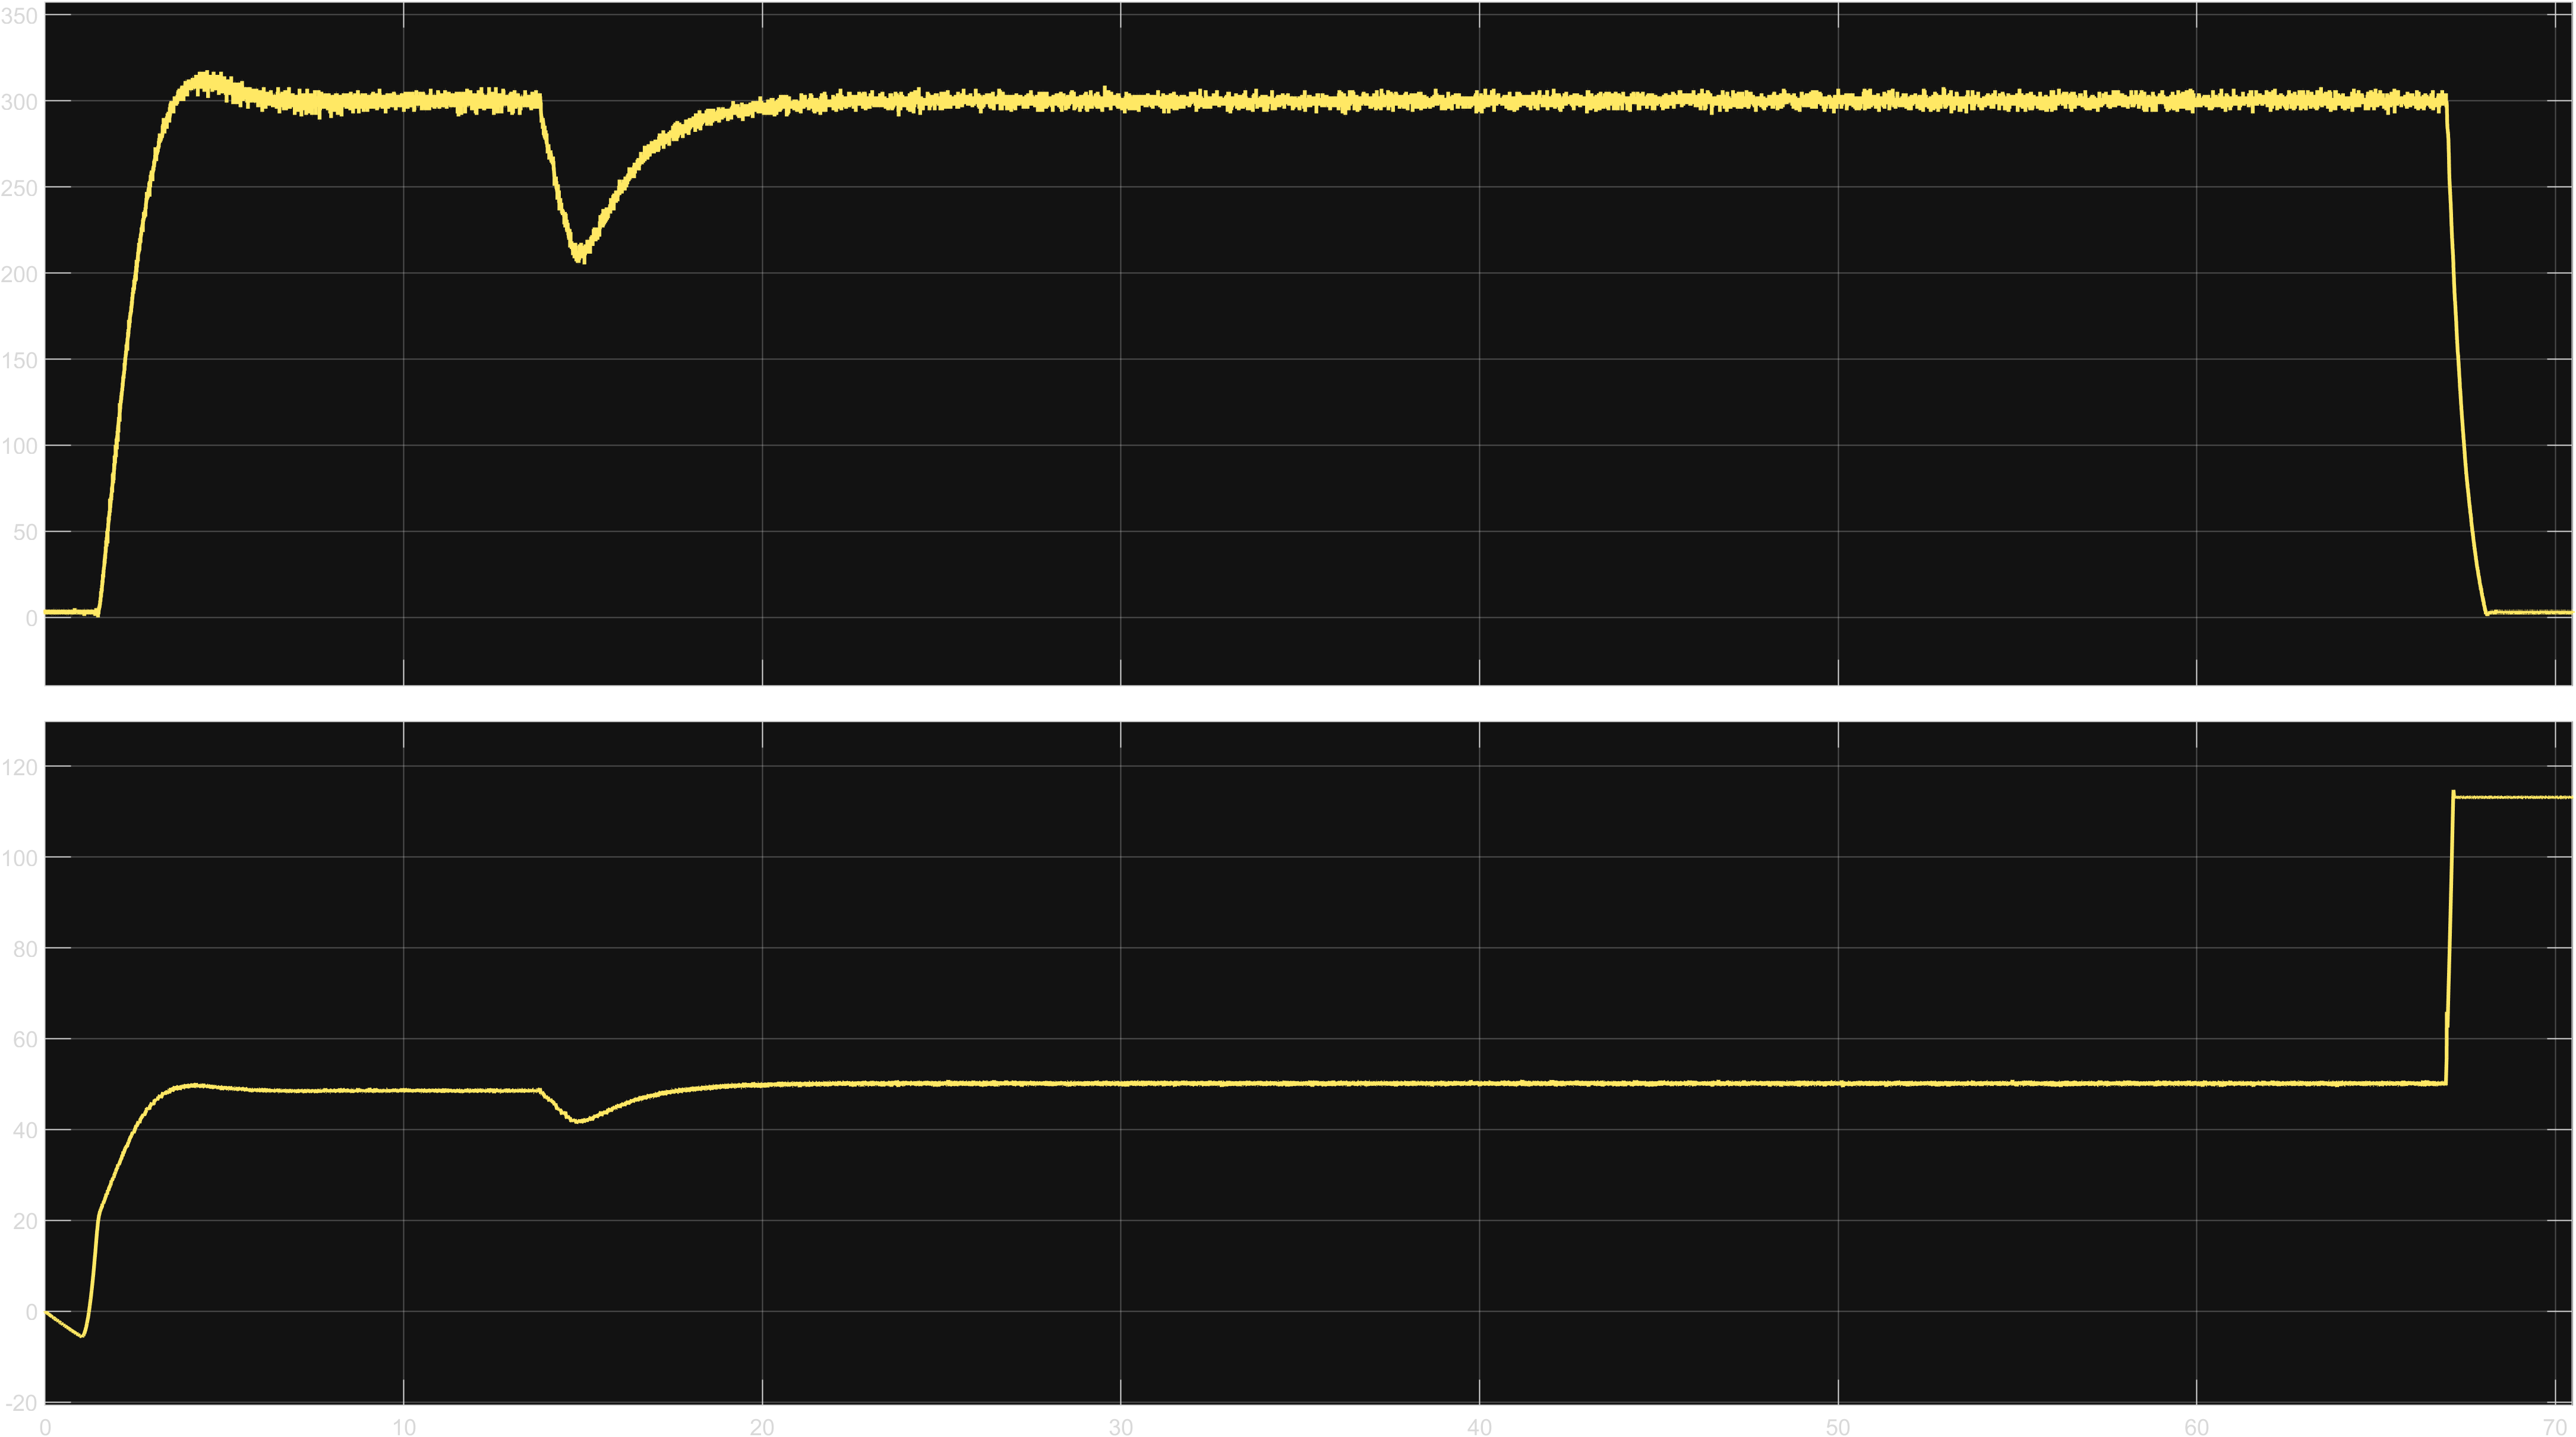
\includegraphics[width=\linewidth, keepaspectratio]{figures/pw.png}
    \caption{Observer validation --- comparison between measured and estimated variables (top: current , bottom: speed).}
    \label{fig:exp_obs_results}
\end{figure}


\newpage
%------------ Conclusion ----------------

\section{Conclusion}
The experimental validation confirmed that the control structures developed in simulation work effectively on the real DC drive, with minor adjustments to account for hardware and safety constraints. 
The current and speed control loops both met the steady-state and dynamic specifications, demonstrating good robustness against disturbances.

The observer-based approach was successful in simulation and partially in the laboratory. 
The current estimation was accurate, but the torque estimation was affected by measurement noise, leading to instability when used for disturbance compensation. 
This highlights the practical challenges of implementing sensorless control on real hardware.

Overall, this practical work successfully connected theoretical modeling, simulation, and experimental implementation. 
It demonstrated the fundamental principles of cascaded control and observer design, and showed how these techniques can be adapted for real-world electrical drives, where nonlinearity, friction, and converter effects must be carefully handled to ensure system stability and precision.






\newpage
%------------ Additional Examples ----------------

\section{Additional Examples}



%------------- Useful Commands ----------------

\section{Useful Commands}

Here are some useful commands:

%------ To insert and cite a centered image -----

\insererfigure{logos/logoCS.png}{3cm}{Figure caption}{Figure label}
% First argument is the path to the image
% Second is the image height
% Third is the caption
% Fourth is the label

Here, I cite the image \ref{fig: Figure label}


%------- To insert and cite an equation --------------

\begin{equation} \label{eq: example}
\rho + \Delta = 42
\end{equation}

Equation \ref{eq: example} is cited here. 



\end{document}